\documentclass[10.5pt,a4paper,twoside]{report}   % list options between brackets

%layout
%\usepackage[left=1.5in, right=1.0in, top=0.5in, bottom=0.5in]{geometry}
%\usepackage[cm]{fullpage}
\usepackage[headheight=10cm,margin=10in,bottom=10in]{geometry}
%\usepackage{layout}
%end

\usepackage{titling}  % list packages between braces
\usepackage{hyperref}
\usepackage{color}
\usepackage{graphicx}
\usepackage{epstopdf}
\usepackage{wrapfig}
\usepackage{pbox} % allows lines in cell
\usepackage{amsmath}
\usepackage{amssymb}
\usepackage{xfrac}
\usepackage{amsthm}
\usepackage{algorithm2e} % for algorithm
\usepackage{alltt} %fancy verbatim
 \renewcommand{\ttdefault}{txtt}
\usepackage[section]{placeins}
\usepackage{listings} %allows for code
\usepackage{color}
\usepackage{gensymb}
\usepackage{bigfoot} %allows verb in footnotes
\usepackage{csvsimple} %allows csv files
%custom colors
\definecolor{mygreen}{rgb}{0,0.6,0}
\definecolor{mygray}{rgb}{0.5,0.5,0.5}
\definecolor{mymauve}{rgb}{0.58,0,0.82}
\definecolor{dark-gray}{gray}{0.3}
\lstset{ %
  backgroundcolor=\color{white},   % choose the background color; you must add \usepackage{color} or \usepackage{xcolor}
  basicstyle=\footnotesize,        % the size of the fonts that are used for the code
  breakatwhitespace=false,         % sets if automatic breaks should only happen at whitespace
  breaklines=true,                 % sets automatic line breaking
  captionpos=b,                    % sets the caption-position to bottom
  commentstyle=\color{mygreen},    % comment style
  deletekeywords={...},            % if you want to delete keywords from the given language
  escapeinside={\%*}{*)},          % if you want to add LaTeX within your code
  extendedchars=true,              % lets you use non-ASCII characters; for 8-bits encodings only, does not work with UTF-8
  frame=single,                    % adds a frame around the code
  keepspaces=true,                 % keeps spaces in text, useful for keeping indentation of code (possibly needs columns=flexible)
  keywordstyle=\color{blue},       % keyword style
  language=Python,                 % the language of the code
  morekeywords={*,...},            % if you want to add more keywords to the set
  numbers=left,                    % where to put the line-numbers; possible values are (none, left, right)
  numbersep=5pt,                   % how far the line-numbers are from the code
  numberstyle=\tiny\color{mygray}, % the style that is used for the line-numbers
  rulecolor=\color{black},         % if not set, the frame-color may be changed on line-breaks within not-black text (e.g. comments (green here))
  showspaces=false,                % show spaces everywhere adding particular underscores; it overrides 'showstringspaces'
  showstringspaces=false,          % underline spaces within strings only
  showtabs=false,                  % show tabs within strings adding particular underscores
  stepnumber=1,                    % the step between two line-numbers. If it's 1, each line will be numbered
  stringstyle=\color{mymauve},     % string literal style
  tabsize=2,                       % sets default tabsize to 2 spaces
  title=\lstname,                   % show the filename of files included with \lstinputlisting; also try caption instead of title
  basicstyle=\ttfamily\scriptsize
}


\hypersetup{colorlinks=true, linkcolor=black  ,urlcolor=blue}
%to add numbered bibliography
\usepackage{etoolbox}


%make better subitem
\let\OldSubItem\subitem
\def\subitem{\OldSubItem \hfill\vspace{-0.6cm}\\ }

%make graphs
\usepackage{pgf}
\usepackage{tikz}
\usepackage[utf8]{inputenc}
\usetikzlibrary{arrows,automata}
\usetikzlibrary{positioning}
\tikzset{
    state/.style={
           rectangle,
           rounded corners,
           draw=black, very thick,
           minimum height=2em,
           inner sep=2pt,
           text centered,
           },
}
%end of make graphs
\makeatletter
\patchcmd{\thebibliography}{%
  \chapter*{\bibname}\@mkboth{\MakeUppercase\bibname}{\MakeUppercase\bibname}}{%
  \chapter{References}}{}{}
\makeatother

\usepackage{fullpage}
\newcommand{\subtitle}[1]{%
  \posttitle{%
    \par\end{center}
    \begin{center}\large#1\end{center}
    \vskip0.5em}%
}           
\newcommand{\email}[1]
{\href{mailto:#1}{\texttt{#1}}}      

\newcommand\Chapter[2]{
  \chapter[#1: {\itshape#2}]{#1\\[2ex]\Large\itshape#2}
}
%for tables
\newcommand{\specialcell}[2][c]{%
  \begin{tabular}[#1]{@{}c@{}}#2\end{tabular}}


\renewcommand{\abstractname}{Executive Summary}
\renewcommand{\bibname}{References}
\renewcommand{\chaptername}{Section}


% type user-defined commands here

\begin{document}
\newgeometry{margin=1.75cm}
\title{\Huge{The EE3 Smart House}}   % type title between braces
\subtitle{Exploring the application of machine learning in the context of home automation}


\author{
  Grubb, Sebastian\\
  \email{sg3510@ic.ac.uk}
  \and
  Murray, Michael\\
  \email{mm510@ic.ac.uk}
  \and
  Janssen, Loek\\
  \email{lfj10@ic.ac.uk}
  \and
  Zhao, Tony\\
  \email{tz1010@ic.ac.uk}
  \and
  Mason, Jonathan\\
  \email{jhm210@ic.ac.uk}
  \and
  Singleton, Matthew\\
  \email{ms8210@ic.ac.uk}
  \and
  van Beek, Jonathan\\
  \email{jv510@ic.ac.uk}
  \and
  Hepburn, Connel\\
  \email{ch3810@ic.ac.uk}
}         % type author(s) between braces
\date{\today \\ Deptartment of Electrical and Electronic Engineering\\ Imperial College London \\ London SW7 2AZ}
\maketitle


\begin{abstract}
With modern societies continued demand for energy, dwindling natural resources and rising prices, technologies that can curb wasteful expenditure are becoming ever more relevant. 
In 2009, 28\% of the total energy produced in the UK was consumed by households, 65.7\% of which was derived from heating alone. Therefore there is a need for a product which can improve the efficiency of household central heating systems, and as a by product save people money. Our solution is an automated system which not only adjusts the home environment to suit the needs of the user, but also minimises wasteful energy consumption. With a unique machine learning approach, the system we propose in this report aims to revolutionise the way in which home environments are controlled.

The scope of existing home automation systems is varied, some providing only remote control while others just data processing. Autohome is a fully integrated system using a unique machine learning approach, that not only automates thermostat settings, but also provides user interaction and remote appliance control. As a result Autohome offers a more comprehensive service that any of its competitors, presenting its users with greater functionality and potential energy savings.

The Autohome solution can be broken down into two key layers;  hardware and software. The hardware layer consists of a network of sensors situated in the users home that collects data on the internal conditions. The software layer sits on a server and processes the collected data to infer thermostat predictions. User interaction with the system is achieved through a mobile app and website. This allows the user to manually adjust the thermostat, remotely control appliances and view feedback statistics on their financial and energy expenditure. As a byproduct of making the user more aware of their energy usage, Autohome should encourage users to become more energy conscious.

Home automation is an emerging market which is expected to grow 16.1\% year-on-year worldwide. However, for example, currently only 0.1\% of UK and 5\% of US homes have a home automation system. Therefore there is huge untapped potential in this market, with as yet no cemented market leader. Considering this, and also combining modern society’s concerns over fossil fuel emissions with the current trend in smart interconnected devices, the conditions are ideal for Autohome to enter the market. 
\end{abstract}



\tableofcontents
\Chapter{Introduction}{Problem Identification and Market Feasibility}            % chapter 1
\section{Problem Identification}     
Modern society's continued and growing need for energy, combined with dwindling fossil fuel reserves and environmental concerns around CO2 emissions, has created an environment in which technology that can limit the wasteful expenditure of energy can thrive.  In 2009 UK households consumed 501TWh accounting for 28-32\% of the UK's total energy expenditure \cite{GBFactFile}. Central heating undeniably plays its role here, and following the current trend of a 3.7 degree centigrade rise in the internal temperature of houses since 1970\cite{DOE2008} ,and rising numbers of UK households its contribution is only set to increase.  As a result there is a need for products that can improve the efficiency of a household heating system.

Current household heating systems are controlled manually via a thermostat, which is neither convenient for the user or sensitive to the actual environmental conditions. In today's busy world few people have the time or discipline to consistently alter their thermostat to fit their own dynamic schedule or the variable nature of the weather. This is not only wasteful in terms of energy but is also very expensive. Therefore there is a niche for a system that can learn and adapt to the chaotic nature of people's lives and the weather.  

The proposed solution to this problem is to create a machine learning system that once trained by the user, intelligently checks whether the occupants of the house are in, out or asleep; and sets the thermostat setting in accordance with this and the external conditions. This system should therefore save energy and make the user experience more convenient while not compromising on  the comfort of the user. As a by product of saving energy the system should also save the user money in the long term; an important consideration is that in the UK 2.6 million households are in fuel poverty, and hence spend at least 10\% of their income on heating \cite{DOEFP2013}. 
\section{Market and Product Feasibility}
Objects are increasingly gaining the ability to communicate and sense their environment, forming what is broadly defined as the Internet of Things. This ability to collect and transmit a vast amount of data in real-time gives rise to new insights, allowing for better day-to-day decisions to be made.

The home automation market forms a subset of the Internet of Things market, with both expected to grow worldwide in 2013 with a CAGR of 16.1\%\cite{mandmhomeauto} and CAGR\footnote{Compounded Annual Growth rate} of 33.2\%\cite{mandmiot} , respectively. Thus it is the ideal time to build a home automation product when so many enablers exist.
\subsection{Product Feasibility}

The first enabler of a home automation product is the reduction in cost of low power processing components. For example the processor used for AutoHome costs \textsterling 6.39 per unit\cite{farnellnxplpc}, with sensors often costing less than \textsterling 1 which means that when assembled an affordable sub \textsterling 150 build price is expected. The second enabler is the increased penetration of smartphones and wireless technology that allows the possibility of an elegant home automation implementation, along with increased consumer demand for such technological solutions. Thirdly is the rise of cloud computing which is the main enabler of AutoHome, as data collected in real-time cannot be as efficiently processed on the mbed as the dataset becomes larger (sensor data being sampled at 5 minute intervals leads to 8640 data-points per house per month) - this is especially true of the computationally intensive machine learning algorithms. Computations are instead done on remote servers(such as Amazon's EC2 compute solution used for AutoHome), which are often more powerful and manage computing loads more efficiently. Additionally current server solutions offer competitive rates priced at \$0.060 per hour and above, relatively affordable operating costs for computing power.
\subsection{Market Feasibility}

With 17.5 million owner occupied homes in the UK and 87.4 million owner occupied homes in the US the home automation market has a huge potential. However only 0.1\% and 5\% of homes, in the UK and US respectively, have such home automation systems. This poor market penetration is due to multiple factors - such as the current state of home automation products, with many of them only offering remote automation and not smart automation. The key difference being that remote automation requires constant human interaction to control the house's settings (though scheduling is possible it is not truly smart), whereas smart automation provides a frictionless experience, constantly adapting to the user's needs. A second reason is the high prices (over-\textsterling 300) of currently available systems\cite{houzzelgan}, which are also described as clunky and tiresome to install. Thirdly is the lack of incentives, as most systems merely act as an additional way to control the house - which amounts to paying a premium to install extra light switches. There is thus little value seen in the cost of such devices, leaving room for a category of affordable, frictionless and smart home automation products which give the consumer clear value - such as saving money and energy.

Additionally recent UK policy has mandated that all UK energy providers must retrofit a smart meter in homes by 2020\cite{hmgovenergy}, meaning there is an additional market involving teaming up with energy providers to provide such systems.

The main market segments are homeowners, where retrofitting this device will be necessary. The other major segment is that of new homes, where there is a focus on delivering modern and energy conscious habitats - meaning that a deeper integration is possible, leading to even more efficient system.
\subsection{Competitors}

Many companies exist in the home automation market, such as AMX, Control4, iControl Networks and Vivint. However most of these only offer remote automation, as explained earlier, though they cover more components of a house, such as window shutter, TV control, house music and personal CCTV.  The table below gives a breakdown.

\begin{center}
    \begin{tabular}{ | l | p{2.25cm} | p{3cm} | p{2.5cm} | p{2.5cm} | p{2.75cm} |}
    \hline
    & \bf AutoHome & \bf Control4 & \bf Vivint& \bf Nest Thermostat&\bf Opower\\ \hline
    \bf{Cost} & \textsterling 150-\textsterling 200 & $<$\textsterling 650 & Starts at \textsterling 38/month&\textsterling 161 & N/A (B2B company)  \\ \hline
    \bf{Features} & -Smart thermostat\newline -Advanced house state detection\newline-lighting and smart meter offered\newline-focused on energy savings\newline -easily installable & -Availability by modules (starter kit \$1000)\newline -Work across residential, commercial and hospitality industries\newline -Offer in depth control including security solutions\newline -Requires contractor for installation & -Offer Home Automation, Energy Management and Home Security solutions\newline -Provide intuitive solutions\newline -No real “smart” automation\newline-Requires contractor for installation &-Smart temperature control\newline -Strong brand in part due to being made by ex-Apple engineers\newline -Focused on saving money\newline -Does not require contractor for installation & -Very good at energy analytics\newline -Sold via energy companies\newline -Provides intelligent software for thermostats \newline -Purely focused on energy  \\ \hline
      \bf{Comparison} & N/A & AutoHome smarter, focusing more on energy saving features &  Smarter than Control4 but not to the extent AutoHome offers, no monthly fee for AutoHome. &  Possibly main competitor. Offers similar “intelligent” algorithms but does not use as much data to regress on as AutoHome.& Competes on the algorithm/machine learning side but offers no other home automation solutions.\\ \hline
    \end{tabular}
\end{center}

\chapter{Top Level Design} 
%graph

\begin{figure}[h!]
  \vspace{-50pt}
  
  \centering
    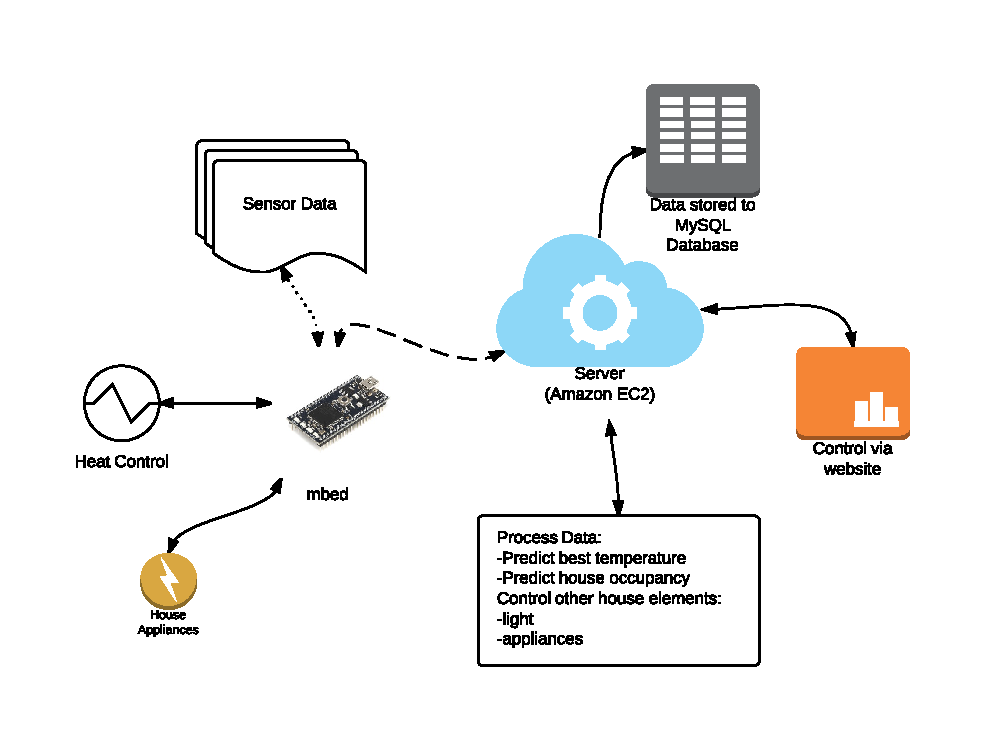
\includegraphics[width=1\textwidth]{images/sysdiag.pdf}
    \caption{Overall System Design}
  \vspace{-10pt}
\end{figure}
%endgraph


\chapter{Modular Design} 
\section{Hardware}     % section 3.1
For the first stage a prototype would be developed, which would include temperature and humidity measurement; an xbee module and a control interface; as well as the ability for the microprocessor to connect to the internet. To facilitate prototyping an 'mbed', prototyping board was used. This board is similar to a microcontroller breakout board but with many extra features, including a USB to FTDI connection for ease of programming, reset buttons and LEDs. This allowed for quick development and allowed basic prototyping to go ahead at an early stage.  Each module was then developed in isolation using the mbed board, and then the final programme was written to combine the various elements together, after which the final link up of software and hardware was devised.
\subsection{mbed}
\begin{wrapfigure}{h!}{0.5\textwidth}
  \vspace{-40pt}
  \begin{center}
    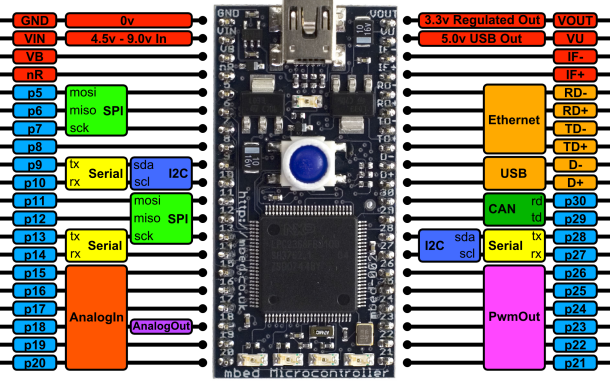
\includegraphics[width=0.48\textwidth]{images/mbed.png}
  \end{center}
  \vspace{-20pt}
  \caption{mbed NXP LPC1768 pinout diagram}
\label{fig:mbed}
  \vspace{-30pt}
\end{wrapfigure}
The 'mbed' prototyping board contains an LPC1768 processor which is a 32-bit ARM cortex-M3 microcontroller\cite{mbeddatasheet}  and the board can be powered either through a USB connection or a 4.5-9.0V input voltage. Figure \ref{fig:mbed} shows the various pins that are available with the mbed board, including a regulated 3.3V supply voltage which is used to power several of the main components. 
\subsection{Wireless Communications}
As discussed in the top-level design, two wireless protocols would play pivotal roles in bringing the entire system together, with the standard wireless local area network (or Wi-Fi) to communicate with the internet via wireless routers which are now found within over 70\% of UK households \cite{homewifi}. Then the xbee protocol was used to communicate with the various sensors and components around the house back to the microprocessor, due to both its low-power usage and the ability to easily create mesh networks. The mbed could then be used to pass the information and commands between the two networks (and hence our servers) as required.
\subsubsection{Wi-Fi}
As stated above there is a reasonable expectation that any home buying our smart thermostat will have wireless internet, both due to the target market and the high proportion of households with wireless routers.  The roving networks Wifly RN-XV module was chosen due to its easy integration into the mbed system and the ability to easily call an ultra-low sleep mode during periods of decreased activity. One slight disadvantage was the inability of the module to join enterprise security networks at the current moment of time, with an updated firmware expected to make such connections possible within a year.

The Wifly module was then set up as shown in the overall circuit diagram (Appendix Section \ref{sec:wificonnect}), using one of the 3 serial pair (RX and TX) connections available on the mbed. Simple ASCII commands using a serial console (in this case PuTTY) were used to experiment with the Wifly module, allowing demonstrable access to the internet which was tested using several standard ISP provided home routers. 

Communicating with the server could be done via several methods, such as http and the new websockets. Both protocols were experimented, with websockets ultimately being chosen, this was due to the ability to have constant 2-way communication between the mbed and server, which could be set-up simply and easily. Using pre-existing libraries the correct SSID and WPA2-PSK code was placed in the Wifly, and then at the beginning of the programme the module is commanded to join the network (see appendix for code). One disadvantage that was found was that if the module failed to join a network over several resets (of the mbed) it would crash and have to be rebooted, either by power cycling or using command mode via PuTTY.
\subsubsection{XBee}
The XBee modules plays a paramount role in servicing communications between all the individual sensors and the MBED which is at the heart of everything. We chose the XBee as we believed that it provided the best features for our design. The XBee ZNET protocol can be used created a mesh network from all of the XBees. This is ideal for application in a household environment where consumers could add extra sensors which could possibly be placed a significant distance away from the central unit.

\begin{wrapfigure}{h!}{0.3\textwidth}
  \vspace{-20pt}
  Legend:\\
  C - Coordinator\\
  R - Router\\
  E - End device
  \begin{center}
    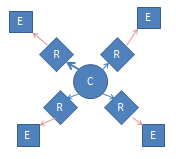
\includegraphics[width=0.28\textwidth]{images/xbeemesh.png}
  \end{center}
  \vspace{-20pt}
  \caption{Diagram depicting the arrangement of the mesh network.}
\label{fig:xbeemesh}
  \vspace{-10pt}
\end{wrapfigure}

Figure \ref{fig:xbeemesh} helps show how the mesh network operates. Our design incorporates one XBee co-coordinator on the central unit with all of the peripherals being configured as router XBees. The XBees which we used had the specifications listed below; the model which was used is the standard XBee not the XBee PRO.

The XBee specifications allow a 40m indoor range which is more than enough to cover most households. On top of this is the fact that each XBee can use it's 40m range to form a mesh network allowing us to greatly increase the effective range of the network. The transmission power is far less than the WiFly equivalent. The power of the XBee is only 2mW even in boost mode vs. an average transmission power of 446mW of the lowest output power rating on the WiFly module in 802.11g mode.

There are two modes of communication to the XBee module, one is called transparent mode or AT mode and the other is the API (Application Programming Interface) mode. Our design is based upon the API mode as it allows greater flexibility and is significantly faster. This could be seen that when issuing commands to the XBee via AT, such as a change to a digital output pin level, there would be a noticeable amount of lag until transition occurred which was not found with API firmware. One other option which the API firmware provided the ability to easily address individual XBees in order to send them commands. This is critical as unique commands are associated with each peripheral type. The AT firmware requires that two registers be set with separate commands to change the destination address when sending to a specific XBee. This creates additional processing load for both the XBee and the central processing unit as well as reducing the speed at which commands can be sent to the XBees. API mode allows 64 bit addressing of XBees within an API frame, allowing a more efficient and convenient method of sending commands with the API framework.

The XBee uses a custom API framework which we created for the purposes of this project. This allows the MBED to construct basic API frames and send them out over its UART port. We have currently only implemented the frames which are required for our project to work though as it is a time consuming process to write and test the operation of a specific command. Currently the framework supports: Requests for the PAN ID, Changing the PAN ID, Sending data packets to other XBees, Requesting the value of all analogue and digital input pins, setting digital levels on the digital output pins.

Details of the framework,its use with different modules, the custom developed API and observed issues can be found in the appendix section \ref{sec:xbee}.

\textbf{Limitations and improvements}

Had there been more time to debug and implement a more robust framework it would have been possible to improve it in a few ways. The first is to get a fully working UART interrupt such that everything can then be called on demand and not consume power when its not needed as well as providing more control on the data coming into the servers. This could be useful in order to throttle some of the connections if the server architecture wouldn't be able to handle the load. 
One more interesting thing would be to write custom firmware for the XBees. By doing this we could offload menial tasks from the MBED and put them onto the XBee. This could be useful if we wanted to convert the power calculations from their raw values to their actual values. This could then be offloaded from the MBED. This would help as the MBED uses a lot more power in its current form than one of the XBee modules. The power drawn has been measured at around 0.7W under normal operating conditions which is considerably higher than the XBee. By taking the load off the mbed we can activate and optimise a sleep routine for the MBED.

This can also be further advanced by changing the MBED with another model such as the one based on the Cortex M0+ from Freescale. This would allow even more power efficient operation as long as there was still enough processing power to run everything. The issue with the M0 is that it does have less connectivity options such as UARTs meaning that some external hardware might have to be used to compensate, thereby increasing the cost.

Lastly the MBED has its own RTOS\footnote{Real Time Operating System}. By using an RTOS it would be possible to thread the web socket operations and the xbee operations in order to get more throughput from the microcontroller as well as massively reducing latency as well.This would come in useful with the power routine and its large wait cycle, allowing  the websocket to be serviced in the meantime. This would however increase complexity and thus would have taken more time to implement and debug. 

\subsection{Sensors}
\label{sec:sensors}
\subsubsection{Temperature sensor}
In order to measure temperature an 8-pin digital sensor was used that has a 2 wire serial interface with the microcontroller, using the I2C pins p28 and p27 upon the mbed board. This was the TMP75AIDR from Texas Instruments and for sensing the temperature, the chip itself is used with thermal paths running through the packaging. This is then converted internally to a digital temperature output with an accuracy of $\pm$ 0.5\celsius, which is then communicated to the microcontroller via I2C. 

The I2C is a multimaster bus which allows easy digital communication with multiple devices if required, and hence the slave address must be set using 3 pin inputs which should match up to the chosen address in the software. Setting the 3 pins to ground gives the address {\color{blue} 0x48} which we can see in the temperature configuration section of the code. Using libraries previously developed for mbed, a simple programme was devised (see appendix) which would only use a 9-bit resolution (set in the temperature configuration code) as a resolution of 0.0625\celsius (12-bit resolution) was deemed unnecessary.  The chip itself was an SMD (surface mount device) and hence a small breakout was constructed to allow ease of use with breadboards.


\subsubsection{Humidity sensor}
Within the thermostat algorithm, internal humidity would play a role and so the low voltage HIH-5030 humidity sensor was acquired, also being an SMD model a small breakout board was required once again. The device has only 3 pins, a $V_{cc}$ , ground, and analogue output which when measured can be used to determine the relative humidity (RH) of the atmosphere to $\pm$3\%.

Using the information supplied in the datasheet two equations were identified, one which could supply the sensor RH from the output voltage, and another to determine the true RH as the sensor RH is also affected by the temperature. Hence the temperature sensor is also required, the final equations within the mbed programme were then

\begin{equation}
    SensorRH=\sfrac{\left( \frac{Voltage\times 5}{3.3}-0.1515 \right)}{0.00636} 
\end{equation}	
\begin{equation}	
    TrueRH=\frac{SensorRH}{1.0546 - (0.00216\times Temperature)}  
\end{equation}

The final true relative humidity would then be calculated within the mbed, which would use an analogue-to-digital pin (ADC) to measure the output voltage of the sensor, the result can then be displayed and returned to the servers as required.


\subsubsection{Wireless Power Monitoring}


The ability to monitor the power consumption of a house in real time is useful in both making the user aware of the impact their habits have on their electricity bill and also to justify any saving the auto-home enables. This is by no means a new idea, and the British government, among many others, intend on a smart meter roll out scheme whereby every home in the UK will have a real time power monitor, or "smart meter", by 2020\cite{doecc}. With this same power information, it is also possible to detect the appliances that are running in the house with non-intrusive load monitoring\cite{hartgw} (NILM), which can indicated unnecessary power usage when nobody is in the house, and switch these off to save power. With this considered, a power monitor is a useful part of the system, and was designed to make accurate measurements with minimum power usage and transmit this to the central unit.

Although measuring power seems a trivial exercise, at AC there are many ways of doing it. One way of making the measurement is calculating the power by summing many instantaneous voltage and current products over a period and divide by the number of samples. Although this is probably the most reliable and accurate method, it is also rather computationally intensive for a low powered 8-bit micro-controller. With the assumption that the voltage and current will have a reasonably consistent shape (sinusoidal), another simpler method is to measure the peak-peak voltage and current, and translate to RMS with a constant factor. However, this is quite a large assumption to make, and for many appliances such as switch mode laptop supplies, the current signal will be very different to that of a light bulb, but this will be less significant when looking at the total draw of a house giving an overestimation of the power usage, which isn't a bad thing.

With the peak-peak voltage/current measurements and a constant factor (for true sinusoids $\frac{\sqrt{2}}{2}$), the conversions can be made to RMS and the apparent power calculated from the product of the two. However, to be able to accurately calculate the dissipative real power, or characterise a load in terms of individual appliance signatures, the phase information must also be recorded. Again, for simplicity and ease of debugging, a comparator $\rightarrow$ XOR$\rightarrow$ low-pass filter phase difference detector was used to give a third ADC input corresponding to the angle between the voltage and current. Again, by only a simple constant conversion factor, the angle and power factor can easily be calculated.   
\subsubsection{Motion Sensor}
An important feature of the home automation project is the ability to detect whether there is anyone within the house. To do this we are using multiple passive infrared motion sensors, located within key locations, to monitor movement. This will provide one of the main sources of data for our learning algorithms. 
Our sensor itself is a long range infrared sensor with a detection range of up to 12m. With a detection angle of up to 102 degrees, this ensures that for the average sized house, all motion within a room will be detected (if placed in one corner). After an initial stabilisation time of roughly 30 seconds, the sensor will output a digital high when the detecting target is present and a digital low otherwise. This is fed straight to the XBee and then to the mbed for processing. 

\begin{wrapfigure}{h!}{0.4\textwidth}
  \vspace{-20pt}
  \begin{center}
    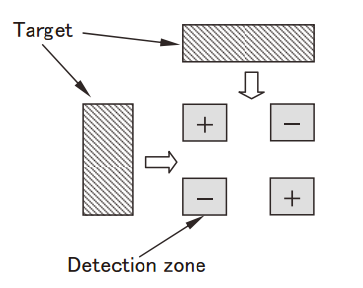
\includegraphics[width=0.38\textwidth]{images/motionsens.png}
  \end{center}
  \vspace{-20pt}
  \caption{Space detection}
  \vspace{-10pt}
\end{wrapfigure}

The method of detection for the sensor is via infrared radiation. This is perfectly suited for human detection from the radiation given out by their body temperature. It also rules out the potential of false triggering from wind blowing on open doors or curtains. However, this does not remove the problem of detection from pets. This is dealt with by the algorithm instead. The sensor consists of multiple polarized detection zones, each zone surrounded by 4 of opposite polarity. When the target moves across these detection zones, the combined polarity varies, hence movement is detected. However, a problem may occur if a target enters a positive and negative detection zone at the same time. In this case the signals will cancel each other and no detection notified. This will usually only occur near the maximum detection range, where the target is smaller in respect to the detection zone. Therefore it is not a significant problem as most rooms would not reach this distance.  

Some other features of the sensor include a metallic can which encloses the sensing circuit. This increases the signal to noise ratio of the sensor. The result provides protection from the false detection of external electromagnetic fields caused by mobile phones and other electronic devices. The simplicity of the device along with the negligible power drawn when no detection is present means that very little total power is consumed during operation. 
\begin{figure}[h!]
  \vspace{-10pt}
  \caption{Motion sensor circuit diagram}
  \centering
    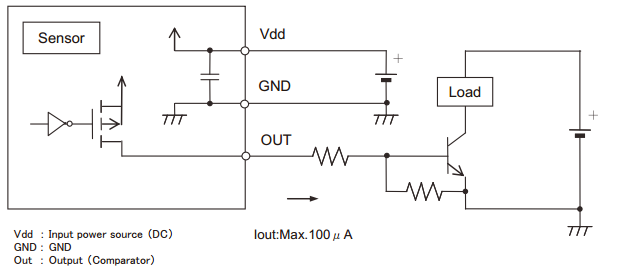
\includegraphics[width=0.5\textwidth]{images/motionsens_diag.png}
\label{fig:motsenscirc}
  \vspace{-10pt}
\end{figure}
The circuit is very simple and can be seen in figure \ref{fig:motsenscirc}. The load is replaced by the XBee and resistor values set to output current/voltage. The input power source is the standard 3.3V used for our XBee and mbed. 

\subsection{Other Hardware}
\subsubsection{Lighting}

As part of the focus to improve user comfort and energy savings, another important feature of the home automation system is the capability to remotely control lights around the house. A large portion of a homeowner's electricity bill is contributed by lighting in the house. In the U.S, this figure is roughly 11 percent of a household’s entire energy budget, and is significantly greater for commercial buildings \cite{DOElighting}. Therefore only keeping the lighting on when necessary can provide substantial savings. 

\begin{wrapfigure}{h!}{0.4\textwidth}
  \vspace{-20pt}
  \begin{center}
    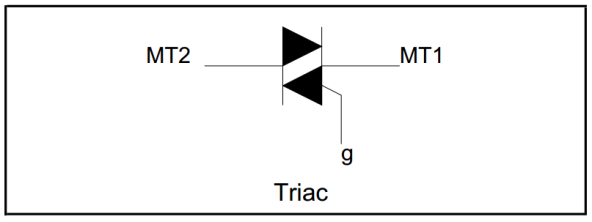
\includegraphics[width=0.38\textwidth]{images/triac.png}
  \end{center}
  \vspace{-20pt}
  \caption{Triac diode diagram}
\label{fig:triac}
  \vspace{-10pt}
\end{wrapfigure}

Our main feature is to keep track of all lighting in the house, allowing the user to see the states of the lights on either an app on their phone or via the website. The user can then change the state of the lights to on, off or auto accordingly. Notifications can also be set to alert the user if any light has been on for a certain length of time. The auto setting will access the motion sensors in the selected room to set those lights to be motion detected. People tend to have various preferences and opinions when it comes to motion detecting lights; therefore our system allows the user full control to choose what suits them best in each room. For example, when in the living room watching TV, the auto setting may not be appropriate as the light will alternate between on/off due to the lack of movement. But the setting can be very convenient for a toilet, as it is used for shorter periods. All these features can ensure no lights are left switched on by accident. 

\begin{figure}[h!]
  \vspace{-10pt}
  \caption{Triac V/I characteristics}
  \centering
    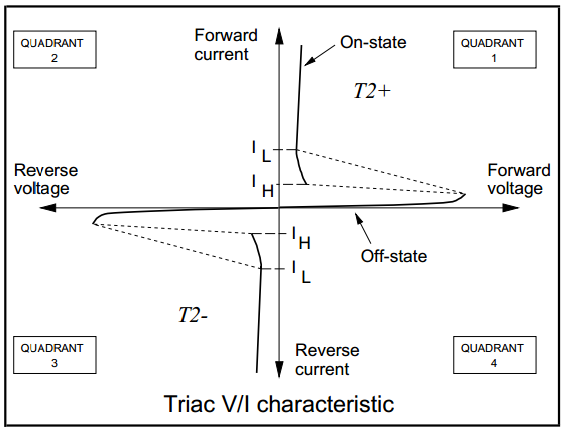
\includegraphics[width=0.5\textwidth]{images/triac_vi.png}
\label{fig:triacvi}
  \vspace{-10pt}
\end{figure}

To remotely control the light switch, we use our mbed to send a signal via the zigbee wireless to an XBee module next to the switch. The XBee will then output a voltage as an input to a XOR gate, with the other being the manual switch located on the wall. Toggling either input will trigger an optoisolator, which will control the high power triac switch, turning it on/off. The triac is connected directly to the mains line of the light bulb, and will conduct only when triggered. The state of the light bulb will then be sent back via the XBee, updating the website and app. 



The characteristics of a triac are ideal for our purpose of switching on/off the mains voltage. As shown in figure \ref{fig:triac}, it is made on two diodes with a gate connection leading from the side of MT1. The function can be comparable to a MOSFET, conducting in either direction when the gate requirements are met. However, unlike the MOSFET, the triac can conduct both AC and DC currents. This is vital as the mains voltage is always an AC. The gate of a triac is triggered by a current, rather than voltage for a MOSFET, and will remain conducting until the current drops below the latching current. For an alternating current, this means the triac will switch off twice every cycle. The V/I characteristics can be seen in figure \ref{fig:triacvi}. 

\begin{wrapfigure}{h!}{0.4\textwidth}
  \vspace{-30pt}
  \begin{center}
    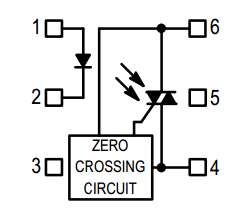
\includegraphics[width=0.38\textwidth]{images/triac_diag.png}
  \end{center}
  \vspace{-20pt}
  \caption{Triac module diagram}
\label{fig:triacmod}
  \vspace{-10pt}
\end{wrapfigure}

To control the gate current of the triac, a zero-crossing optoisolator is used. The zero-crossing section ensures the gate of the triac is switched on when the current reaches 0. This is important as the phase of the current will be zero, so no noise is generated. Without it, switching could occur at peak voltages, which not only would produce EM noise, but also result in a large $ \frac{dV}{dt}$ and potentially blowing the load. The optoisolator also keeps the mains voltage electrically isolated from the XBee circuit. This prevents the mains voltage blowing up the XBee in the case of a short circuit or if the triac blows. Isolation is achieved by simply using an LED to trigger a phototransistor. Hence, the input of the Xbee is attached to pins 1 and 2, and the triac to pins 4 and 6 (figure \ref{fig:triacmod}).

Not only does remotely controlled lighting reduce energy costs, it can also serve as a tool to provide home convenience for users. With a touch of the phone, no-longer do users need to feel around in the dark for the switch to use the toilet at night, or to get out of bed to switch lights off. Because the feature simply controls the mains supply, it can be easily applied to all electronic appliances. TVs, dishwashers and washing machines are just a few examples of common household appliances that are often left on standby. Switching these off when not in use can provide further cost cuts in the long run. 
\section{Software}     % section 3.2
\textit{Note:} Software was developed in parallel of  the hardware, thus no past data collection was available. Instead data made publicly available for the purpose of smart homes research used. The main sources used were the University of Massachusetts Amherst SMART* dataset \cite{umasssmart} as well as Washington State's Tulum dataset \cite{tulumwsu}.
\subsection{Server Architecture and Technologies}
The main server architecture works on a LAMP\footnote{The LAMP acronym  refers to the first letters of Linux, Apache(a HTTP server), MySQL (database solution), and PHP or Python, the main components to build most web servers.} server as this provides the system with a database (MySQL) to store all the collected sensor data, a means of processing this data (Python with the numerical NumPy and SciPy libraries) and easily controlling the system (HTTP server with PHP allowing delivery of interactive web-pages). 

To enable the website to be able to access the data that is stored in the database, such as the predicted timetable or the past weather information, the server-side programming language of PHP was used. This is the language that is generally used for database access on websites, as it has good support for SQL databases and is easily used in conjunction with HTML. All PHP code is also executed on the server, before being returned to the end-user. This makes it useful as the code must include the database username and password, which would otherwise be passed to the user in the source code, giving anyone access to the database and the ability to alter information. PHP can also be used to create session variables on the server, which allows the creation of a basic login system. Again, as the code is executed server side, a redirect to the login page can be made if the user is not logged in, which will be executed before any of the html is loaded.

The only disadvantage of PHP being executed server side is that it cannot be used to write executable functions on the same page, which is needed when making changes to the timetable and a few other parts of the website. However using ajax from the jquery library, we can call other web pages without leaving the current page, and even pass variables to them which provides a solution for us.

PHP is also used for calling the weather API, to get the current weather conditions. The code gets the contents from a specially generated URL that contains the current weather conditions in JSON format. This can then be decoded, making each weather element easily accessible and these can then be stored into a database. This code is then be called every five minutes using a simple python script running constantly on the server.
\subsubsection{Server Software}
To control the system a constantly running program, monitoring, processing and relaying all the messages passed is needed. Thus a server-side program which could both send and receive messages to and from system modules was made.

To pass on messages the websocket technology was used. While a relatively new technology, websockets were chosen for their ideal use in real-time applications. This avoids using old 'hacks' such as using \verb+HTTP+ \verb+POST+ and \verb+GET+ requests\footnote{\verb+HTTP+ \verb+POST+ and \verb+GET+ requests are the traditional way in which webpages get accessed} at irregular intervals to achieve a near-realtime connection. This is because websockets provide a full duplex connection with no need of polling\footnote{i.e. calling the server to ask for a reply} from the client. This would allow the message to turn off a light, or turn the temperature up, to be sent and received nearly instantly - thus being as useful if not more than a real switch.

The main server was written in Python, chosen for its ease of use and good integration with web technologies, using the \href{http://www.tornadoweb.org}{tornado} framework as code base. The server works by receiving messages in \verb+JSON+\footnote{\verb+JSON+ stands for JavaScript Object Notation and is a human readable standard allowing simple data structures to be represented. For example to encode the variable name='Alex' and age=26 the following message would be sent:\verb+{"name":"Alex","age":26}+} and passing them on to the appropriate program. For example if a user, via the website page, requests the current house temperature the server receives it and passes it on to the mbed module. Alternatively if the mbed sends the current sensor data to the server a separate script is called to add the values to a database and process this data to predict the most ideal temperature, for example. All the server code can be found in the appendix section \ref{sec:tornadocode}.

\begin{figure}[h!]
  \vspace{-10pt}
  \caption{Flow diagram of the server's general function}
  \centering
    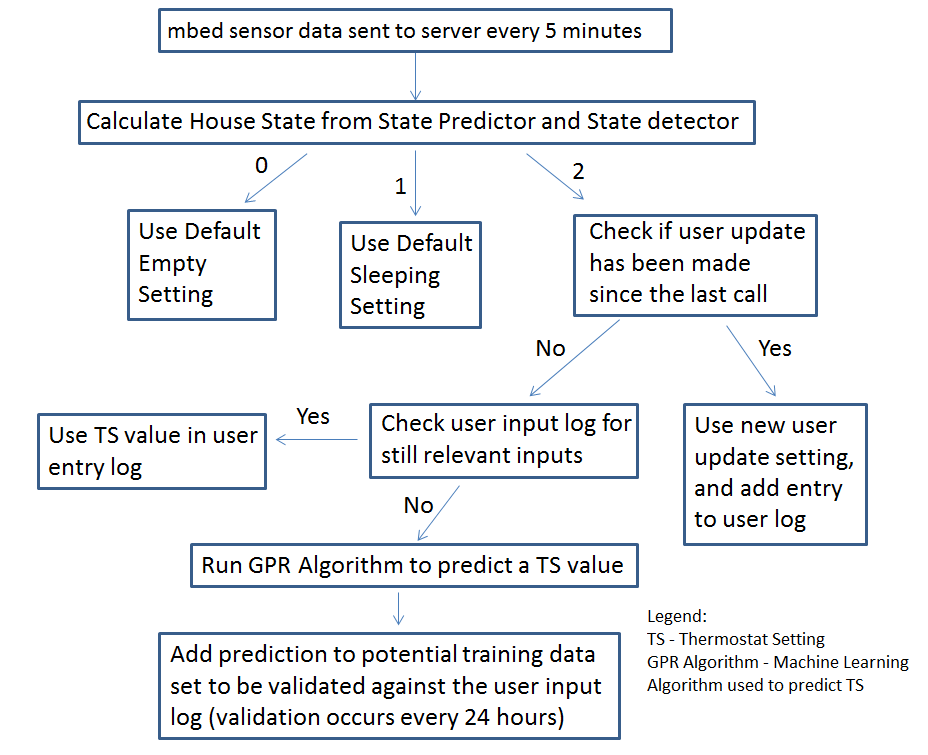
\includegraphics[width=0.6\textwidth]{images/system_overview.png}
\label{fig:sysoverview}
  \vspace{-10pt}
\end{figure}
\FloatBarrier

Figure \ref{fig:sysoverview} is an overview of how the server works when receiving the mbed data to then control the house's thermostat setting.

\subsection{Hidden Markov Model for Occupation State Detection}
\subsection{Timetable Prediction}
\label{sec:ttpredictprog}
While a Hidden Markov Model provides a good way to determine the current state of the house another essential feature to ensure comfort and optimize energy usage is timetable prediction. Different methods were considered such as using the Hidden Markov Model to predict future states, taking an average state of every day of the week or making an ARMA/ARIMA model. The main criteria for choosing a method was an efficient one which could predict to a good degree of accuracy what will happen in about 6 hours in the future. Thus a method suggested by Microsoft Research \cite{msftresearch} was implemented and adapted.

The idea behind the proposed solution is to look at $n_p$ past states to predict the future $n_f$ data-points by finding other similar instances. We thus measure similarity from taking the hamming distance of each time-series vector. Indeed each vector is in the form $\vec{t}_{vp} = [0,1,1,1,2,2,\dots,2,1,0]$, with 0 signifying an away state, 1 a present state and 2 a sleeping state, meaning that taking the Hamming distance between two such vectors is possible. From this a determined number of similar days can be found to use their known future data-points to predict the current future. This is summarized in Algorithm \ref{eq:ttpredict}.\\

\begin{algorithm}[H]
 \SetAlgoLined
 \KwData{Time-series vector of past $n_p$ states - $t_{vp}$}
 \KwResult{Time-series vector of future $n_f$ expected states - $t_{vf}$}
 take current time and give it an index $n_n$\;
 \For{i index of all past days}{
 set $t_{vd}$ equal to the $n_n - n_p$ to $n_n$ data-points of $day_i$ (i..e the same time range than $t_{vp}$ but in the present)\;
 store in $D_i$ the Hamming distance of $t_{vd}$ and $t_{vp}$\;
 }
 get the indices of the 4 closest days in terms of Hamming Distance from $D_i$\;
 from these selected days get the $n_n$ to $n_n+n_f$ data-points\;
 get the mode of these selected days and store in $t_{vf}$\;
 \Return{$t_{vf}$}
 \label{eq:ttpredict}
 \caption{Timetable State prediction}
\end{algorithm}

To find the optimal number of days to use to predict future expected states by taking their mode - i.e. should the closest $x$ or $y$ days be used - various prediction scenarios were run with the results presented in section \ref{sec:daychoice}. They show that, for the used dataset (3 months long), the optimal days to take the mode of was 4 as this consistently gave the highest average accuracy and one of the lowest standard deviations\footnote{Over 3 months worth of data, about 80 days have their future states predicted and the accuracy of each of these instances is recorded, yielding an average and standard deviation for accuracy over different parameters}. 

In deciding how long the vector $\vec{t}_{vp}$(i.e. the length of time to look back into the past to predict the future states) should be a MATLAB script testing for the accuracy of different settings\footnote{This was done by taking the states of each day in a 3 month long dataset separately, removing it from the data set, and trying to predict the future(know to us but unknown to the algorithm) states.}. In Figure \ref{fig:predcons} the results were plotted and suggest that taking the last 12 hours of house states gives us the most insight into the future - with the accuracy varying little with regards to the time looked into the future, except for very short amounts of time or 12 hours onwards which is because a house state is not likely to imminently change and that as we approach 24 hours we approach a day's length which is typically regular in nature.


\begin{figure}[h!]
  \vspace{-10pt}
  \caption{Model of accuracy using time length past values (sample p) compared to the future hours predicted (sample f)}
  \centering
    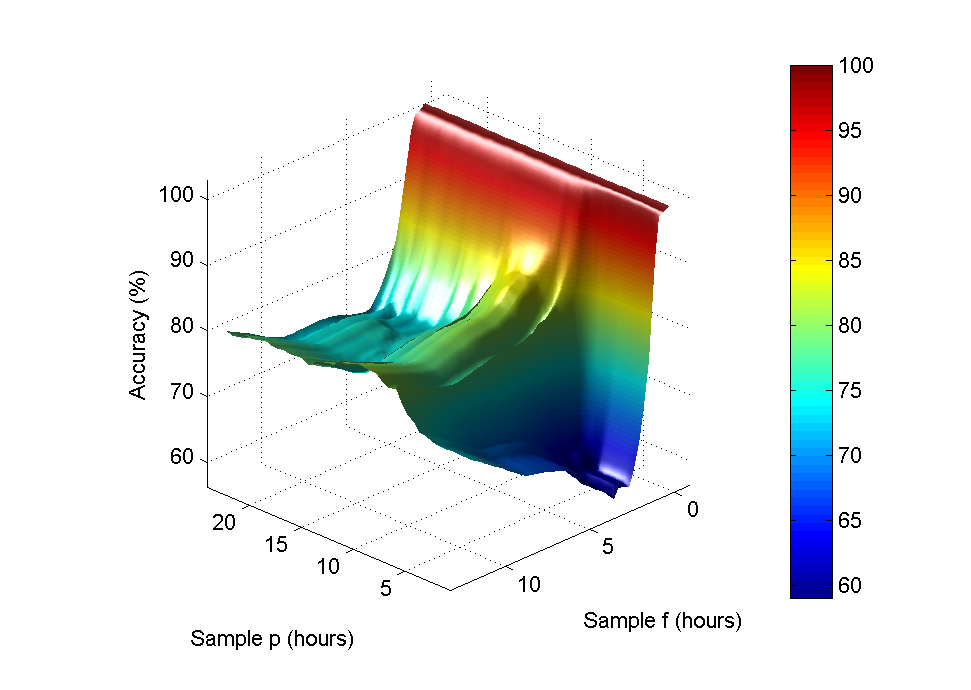
\includegraphics[width=0.7\textwidth]{pred_consideration.eps}
\label{fig:predcons}
\\ \textit{Data used: University of Massachusetts Amherst SMART* dataset \cite{umasssmart}}
  \vspace{-20pt}
\end{figure}
\FloatBarrier
\subsection{Machine Learning for Thermostat Setting Prediction}
A fundamental part of the functionality of the system is the ability to be able to predict the user's desired thermostat setting given the state of the house and external conditions. This can be achieved through a machine learning algorithm, which regresses through the training data provided by the user to predict a thermostat setting given external conditions not present in the training set. Two regression algorithms were developed, and in this section both are discussed.
\subsubsection{Linear Regression}
\begin{wrapfigure}{h!}{0.4\textwidth}
  \vspace{-40pt}
  \begin{center}
    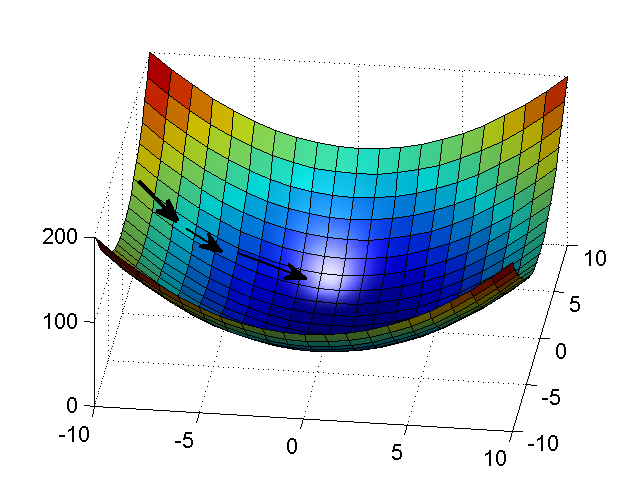
\includegraphics[width=0.38\textwidth]{convexcurve.eps}
  \end{center}
  \vspace{-20pt}
  \caption{A convex cost function}
\label{fig:cvxcost}
  \vspace{-30pt}
\end{wrapfigure}

The initial implementation involved implementing a basic linear regression model to fit past data. This works by finding the parameters of the vector $\vec{\theta}$ which forms the prediction function $h(x,\theta) = \sum\limits_{i=0}^n \theta_i x_i = \theta^T x$ where $\vec{x}$ is the input data and $n$ is the number of parameters. To fit the parameters we have a dataset of $x$'s with it's corresponding values of $y$. From this a cost function $J(\theta) = \frac{1}{2m} \left( \sum\limits_{i=1}^m \left( h(x_{(i)},\theta) -y_{(i)} \right)^2 +\lambda \sum\limits_{i=1}^n\theta_i^2 \right)$ is defined, where $m$ is the number of data-points.Thus by choosing a $\theta$ which closely fits the input data we can see that $J(\theta)$ will be minimized. (The $\lambda \sum\limits_{i=1}^n\theta_i^2$ term is there to ensure that $\theta$'s magnitude is not too large - avoiding the problem of the prediction function not being general enough for future, unknown inputs). Minimizing $\theta$ is a matter of performing a process called gradient descent which involves following the gradient direction. Figure \ref{fig:cvxcost} shows 3 arrows each representing the gradient at 3 different points. It can be seen from this that following the gradient leads to a less steep gradient until a minimum is reach - in which case the gradient will be zero\footnote{This method also works on non-convex functions but will only return a local minima - however $J(\theta)$ is always convex for the case of linear regression}.

Using the SMART* dataset a $\theta$ was found to fit the past data whose features include inside \& outside humidity, outside temperature,wind-speed, time of the day and day of the week with output inside temperature. From this Figure \ref{fig:linreg} was made, where all other features except time and day of the week were kept constant, to give an idea of the type of model created. It can be observed that this current model implies a trend of lower temperatures on weekdays with temperature consistently lower during sleeping hours - which implies that the model works in learning from past house activities.

\begin{figure}[h!]
  \vspace{-10pt}
  \caption{Model of a house's temperature with time and day of the week as variables. Gradient descent was used to fit a 4\textsuperscript{th} order function.}
  \centering
    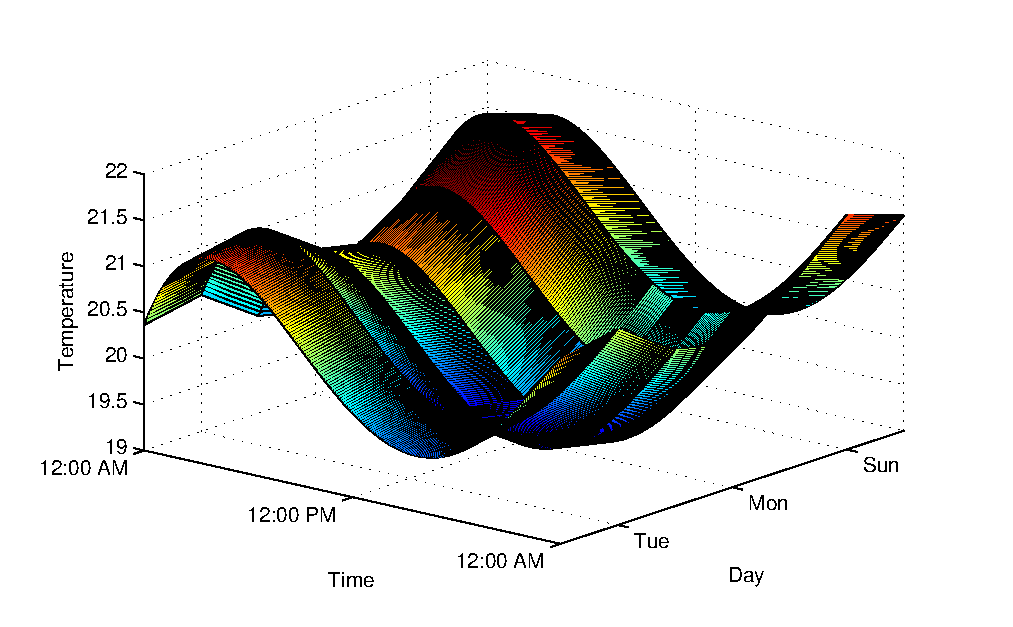
\includegraphics[width=0.5\textwidth]{linreg.eps}
\label{fig:linreg}
  \vspace{-25pt}
\end{figure}
\
\subsubsection{Gaussian Process Regression}
\label{sec:gprmltemp}

The issue with using 'non-Bayesian paradigm' algorithms, i.e. ones that typically assume no prior distribution or structure on a hypothesis,  is that the regression curve is found (or trained) by minimizing the empirical error.  However what is actually desired is to minimize the error on future predictions. This requires a Bayesian setting \cite{MITGPRbook, edsnelgpr}.

	Using a Bayesian setting a structure or prior is assumed, which, in the case of GPR, is a Multivariate Gaussian distribution \cite{MITGPRbook,StanfordStats}.  Parametric techniques, for example linear regression, restrict the class of functions which can fit the training data and then optimize parameters by minimizing the error between the target data set and the predicted values\cite{MITGPRbook,dukegpr}. GPR in contrast allows every possible function but gives each a prior probability, which can then be used to calculate a posterior probability once the training data has been taken into account. In this way then we can think of the GPR as filtering the functions in terms of their likelihood given the training data. As a result, while parametric techniques can generate curves that closely fit the data, only Bayesian techniques like GPR can quantify the expected error and therefore work to minimize it\cite{MITGPRbook,GPMLDoc,GPROpt,scikitlearn}.

\noindent \underline{\textbf{Notes on Notation:}}

In this section, bold font indicates vectors and matrices while non-bold indicates scalars and functions. If a character denotes a function then the emboldened version of the same character represents a set or vector of elements taken by evaluating that function at certain points:

\begin{itemize}
\item Features vectors are denoted by $\boldsymbol{x}$. 
\item The training data is a set of feature points. In matrix form it is denoted by $\boldsymbol{X}$ and represents a collection of feature vectors. '$n$' is the number of training examples in our training set.
\item $f(\boldsymbol{x})$  (or,in suppressed argument form,$f$) is the hypothesis function we wish to infer. $f^\ast$ is the prediction we want to make about the function $f(\boldsymbol{x})$ evaluated at a point $\boldsymbol{x}^\ast$ not present in the training set. 
\item $y(\boldsymbol{x})$ (in suppressed argument form as $y$) is the function of observed thermostat results, i.e. the underlying function we wish to infer plus a noise term: $y(\boldsymbol{x})=f(\boldsymbol{x})+\epsilon$, where $\epsilon \sim \mathcal{N} (0,\sigma_{n}^2 \boldsymbol{I})$ is Independent Additive White Gaussian Noise (IAWGN) with $var(\epsilon)=\sigma_{n}^2$. The target data of the training set is denoted by y and is simply a vector of elements of $y(\boldsymbol{x})$ evaluated at different points.
\item '$\theta$' Indicates the hyperparameters that are used to define the covariance function, in vector form this is denoted '$\boldsymbol{\theta}$'.
\end{itemize}

It is important to bear in mind that a vector or matrix is a way of expressing a set of data points. If these data points are random then this data set can be written as a random vector or matrix whose elements are random variables each with a probability distribution, which in the case of GPR is Gaussian.  As a result data sets, made up of a collection of random variables each with a Gaussian distribution can be expressed as a multivariate Gaussian distribution.

\noindent \underline{\textbf{Prior and Hyperparameters:}}

As previously discussed GPR is a non-parametric technique, which makes it a powerful tool as no assumptions need to be made on the hypothesis function directly, instead only on the probability distribution of the hypothesis function. The reason that GPR is a good choice in this case is because Gaussian distributions are continuous (important as the hypothesis function we wish to infer is continuous) and flexible. The prior for GPR is defined as:

\begin{equation}
    f \sim GP(\boldsymbol{0},k \left( \boldsymbol{x_i},\boldsymbol{x_j} \right))
\end{equation}	

The above equation states that without any information the distribution of possible hypothesis functions is defined by a Gaussian Process with a mean function of 0 and a covariance function k.  As a result to specify the Gaussian prior all that is required is to describe its covariance function (since the mean function can be set to 0 without any loss of generality) \cite{MITGPRbook}
. The kernel deployed in this particular application is the squared exponential, also called the Gaussian Kernel, with an added noise term \cite{MITGPRbook}:

\begin{equation}
    k \left( \boldsymbol{x_i},\boldsymbol{x_j} \right)=\sigma_{f}^2 \exp\left(-\dfrac{1}{2} {\left( \boldsymbol{x_i}-\boldsymbol{x_j} \right)}^T \boldsymbol{M} \left( \boldsymbol{x_i}-\boldsymbol{x_j} \right)\right) + \sigma_n^2 \boldsymbol{\delta_{ij}}
\end{equation}	

$\boldsymbol{x_i} \text{ and }\boldsymbol{x_j}$\textbf{ }are input feature vectors,  ${\sigma }^2_f$ is the `signal power' which represents the overall scale variation of the latent (not yet manifested) thermostat setting. ${\sigma }^2_n$ is the `noise power' representing the noise variation or `jitter' in the data \cite{dukegpr}. Physically this is the manifestation of the users own error in their thermostat setting. For example, on a particularly cold day the user may be tempted to initially turn up their thermostat setting beyond what they actually find comfortable or need. ${\delta }_{ij}$ is the Kronecker product, meaning that the noise term is only added to the variance of a point\cite{dukegpr}. This is due to the nature of the noise being IAWGN i.e. the noise on different samples is independent. Finally M is a diagonal matrix containing the length scales of each feature \cite{MITGPRbook}:
\begin{equation}
\boldsymbol{M} = \left[ \begin{array}{ccc}
\frac{1}{l^2_1} & 0 & 0 \\ 
0 & \ddots  & 0 \\ 
0 & 0 & \frac{1}{l^2_n} \end{array}
\right]
\end{equation}

Length scales represent the distance in a feature dimension that must be moved before the function value changes significantly. Large length scales imply irrelevant features while short length scales mean that the error in the prediction grows rapidly away from the data points \cite{dukegpr}. Having individual length scales for each feature is more flexible than having just one general length scale as there will be variation in length scales from feature to feature. 

The error squared exponential kernel was chosen as it provides a smooth (infinitely differentiable) hypothesis and is generally the most widely used and applicable kernel in machine learning.

\noindent \underline{\textbf{Hyperparameter Optimization:}}

To achieve accurate predictions the hyperparameters need to be optimized to ensure the model best fits the training data. In this way the task of 'teaching' a Gaussian Process Regressor is therefore equivalent to optimizing the hyperparameters to fit the training data. The marginal likelihood is the 'model evidence' and by maximising the marginal likelihood the optimum hyperparameters can be found (See appendix for more information)\cite{MITGPRbook,GPROpt,camgpr,edsnelgpr}.


The probability of the target data `y' given the training data, hyperparameters and assumed prior distribution is the called the likelihood \cite{camgpr,edsnelgpr}: 
\begin{equation}
P\left(\boldsymbol{y}\mathrel{\left|\vphantom{\boldsymbol{y} \boldsymbol{X}\boldsymbol{,\ }\boldsymbol{\theta },\boldsymbol{f}}\right.\kern-\nulldelimiterspace}\boldsymbol{X}\boldsymbol{,\ }\boldsymbol{\theta },\boldsymbol{f}\right)\ \sim \ \mathcal{N}(\boldsymbol{f},\ {\sigma }^2_n\boldsymbol{I}\boldsymbol{)}
\end{equation}
 This distribution makes intuitive sense considering that $y(\boldsymbol{x})=f(\boldsymbol{x})+\epsilon$  \cite{MITGPRbook,UManMND} and that the any collection of samples drawn from a Gaussian Process naturally has a Multivariate Gaussian Distribution. The marginal likelihood, $P(\boldsymbol{y}\boldsymbol{|}\boldsymbol{X}\boldsymbol{,\ }\boldsymbol{\theta })$,  is found by taking the conditional probability of the likelihood given certain values of $f$, and then averaging this by integrating over all values of$\ f$. This is equivalent to taking the expectation:
 
\begin{equation}
P\left(\boldsymbol{y}\mathrel{\left|\vphantom{\boldsymbol{y} \boldsymbol{X}\boldsymbol{,\ }\boldsymbol{\theta }}\right.\kern-\nulldelimiterspace}\boldsymbol{X}\boldsymbol{,\ }\boldsymbol{\theta }\right){\rm =}{\rm \ }E\left\{P\left(\boldsymbol{y}\mathrel{\left|\vphantom{\boldsymbol{y} \boldsymbol{X}\boldsymbol{,\ }\boldsymbol{\theta },f}\right.\kern-\nulldelimiterspace}\boldsymbol{X}\boldsymbol{,\ }\boldsymbol{\theta },f\right)\right\}=\ \int{P\left(\boldsymbol{y}\mathrel{\left|\vphantom{\boldsymbol{y} \boldsymbol{X}\boldsymbol{,\ }\boldsymbol{\theta },f}\right.\kern-\nulldelimiterspace}\boldsymbol{X}\boldsymbol{,\ }\boldsymbol{\theta },f\right)P\left(f\boldsymbol{|}\boldsymbol{X}\boldsymbol{,\ }\boldsymbol{\theta }\right)df}
\end{equation}

$P\left(\boldsymbol{f}\boldsymbol{|}\boldsymbol{X}\boldsymbol{,\ }\boldsymbol{\theta }\right)\ \sim \ N\left(\boldsymbol{0}\boldsymbol{,\ }\boldsymbol{K}\right)$ is the probability distribution of the function we wish to infer without any target set. In this way, it is equivalent to simply drawing points from our prior distribution. We can see therefore that both the prior set and the likelihood set are both Gaussian.  The product of two Gaussians is also Gaussian, integrating over $f$ it can be proved that\cite{MITGPRbook}:

\begin{equation}
 \boldsymbol{y}\boldsymbol{|}\boldsymbol{X}\boldsymbol{,\ }\boldsymbol{\theta }\ \sim  \mathcal{N}(\boldsymbol{0},\ \boldsymbol{K}+{\sigma }^2_n\boldsymbol{I})
\end{equation}
 
Referring to the equation for the PDF of a Gaussian Multivariable Distribution, and setting $\boldsymbol{C}=\ \boldsymbol{K}+{\sigma }^2_n\boldsymbol{I}$ the PDF for the Marginal Likelihood (see Appendix) can be defined:

\begin{equation}
P\left(\boldsymbol{y}|\boldsymbol{X,\theta}\right)=\ {2\pi }^{-\left(\frac{n}{2}\right)}{\left|\boldsymbol{C}\right|}^{-0.5}\exp\left(-\frac{1}{2}y^T{\boldsymbol{C}}^{-1}y\right)
\end{equation}

In its current form it is not particularly conducive to the task of optimization. A common and successful technique for optimizing any parameters is to turn the problem into a minimization task, and find a global or acceptably good local minima using gradient descent. Taking the natural log of the equation:

\begin{equation}
\log \left( P\left(\boldsymbol{y}|\boldsymbol{X,\theta} \right)\right)=\ -\left(\frac{n}{2}\right){\log  \left(2\pi \right)\ }-\frac{1}{2}{\log  \left(\left|C\right|\right)\ }-\frac{1}{2}y^TC^{-1}y
\end{equation}

Rearranging and multiplying by negative one we end up with what is known as the 'Negative Log Marginal Likelihood' or NLML \cite{camgpr,edsnelgpr}:

\begin{equation}
-\log  \left(P\left(\boldsymbol{y}|\boldsymbol{X,\theta}\right)\right)=
\frac{1}{2}y^TC^{-1}y +\frac{1}{2}{\log  \left(\left|C\right|\right)}
+\frac{n}{2}{\log  \left(2\pi \right)}
\end{equation} 

Note that by minimizing the NLML we are maximising the Marginal Likelihood and therefore gradient descent techniques can be applied. First the hyperparameters are initialised randomly and then taking the partial differential of the NLML with respect to each hyperparameter the error curve can be traversed (error curve is the NLML as a function of the hyperparameters) to find a minima. Denoting the NLML as $L\left({\mathbf \theta }\right)$ \cite{edsnelgpr}: 

\begin{equation} 
\frac{\partial L\left(\boldsymbol{\theta }\right)}{\partial {\theta }_i}=\frac{1}{2}tr\left({\boldsymbol{C}}^{-1}\frac{\partial \boldsymbol{C}}{\partial {\theta }_i}\right)-\frac{1}{2}{\boldsymbol{y}}^TC^{-1}\frac{\partial \boldsymbol{C}}{\partial {\theta }_i}C^{-1}\boldsymbol{y}
\end{equation} 

A basic gradient descent function can be used to update the hyperparameters by subtracting a value proportional to the partial derivative of the NLML with the hyperparameter in question. Over the process of many iterations, and given an appropriately sized step size$\ \alpha $ (i.e. one that is not too large so as to diverge or too small so as to converge too slowly), the NLML will converge to a point of zero gradient. As we are subtracting this term this convergence limits towards a minima, not a saddle point or maxima:

\begin{equation} 
{\theta }_i={\theta }_i-\ \alpha \frac{\partial L\left({\mathbf \theta }\right)}{\partial {\theta }_i}\ \ 
\end{equation} 

Unfortunately this problem is not convex (i.e. the error curve is not convex) and therefore there does not exist a global minima. Instead there is the potential for many minima and maxima depending on our selection of training data. As a result all that can be hoped for is that gradient descent gives us an acceptable local minimum. 

The convergence point depends on what the initialisation of the hyperparameters; different initialisations lead to different starting points on the error curve and therefore potentially different local minima. The practical approach taken to solve this issue was to perform a grid search over an area of the error curve (that seemed most logical given our instincts on the data), perform gradient at points initialised in divisions of this area and then choose the area that seemed to give the lowest average NLML. The division with the lowest NLML can then be selected as the new area of consideration, and the process can be repeated till an appreciable initialisation range is found. This, and the computational complexity of all the algorithms discussed in this section, is discussed in more detail in the results section. 

\noindent \textbf{\underbar{Intuition behind Gaussian Process Regression:}}

With a Gaussian prior the assumption is made that the space of possible functions that we can use as our hypothesis is normally distributed.  By then observing data, i.e. getting a training set, the distribution can be conditioned on the training set. By then finding the mean or average of this distribution function that best, or most likely fits the user's desired thermostat setting given certain environmental conditions, can be found. Points in the training data set can be seen as anchors in this function distribution having zero variance \cite{MITGPRbook,GPMLDoc,scikitlearn,dukegpr}.

Considering a new input feature vector ${\boldsymbol{x}}^{\boldsymbol{*}}$ 
and a desired prediction about $f(\boldsymbol{x}^\ast )$ ($f^\ast$ for convenience) then adding this point to the training data results in a joint Gaussian distribution \cite{MITGPRbook}:
\begin{equation}
\left[ \begin{array}{c}
\boldsymbol{y} \\ 
{\boldsymbol{f}}^{\boldsymbol{\ast}} \end{array}
\right]\ \sim \mathcal{N}\left(\boldsymbol{0},\ \left[ \begin{array}{cc}
\boldsymbol{K}+{\sigma }^2_n\boldsymbol{I} & {\boldsymbol{K}}_{\boldsymbol{\ast}} \\ 
{\boldsymbol{K}}^{\boldsymbol{T}}_{\boldsymbol{\ast}} & {\boldsymbol{K}}_{\boldsymbol{\ast\ast}} \end{array}
\right]\right)
\end{equation}
Here $\boldsymbol{K}_{\boldsymbol{\ast}} = \begin{bmatrix} k\left(\boldsymbol{x}_{\boldsymbol{\ast}}, \boldsymbol{x}_{\boldsymbol{1}}\right)\\ \vdots\\ k\left(\boldsymbol{x}_{\boldsymbol{\ast}}, \boldsymbol{x}_{\boldsymbol{n}}\right)\end{bmatrix}$ denotes the covariance matrix (or in this case, as $\boldsymbol{x}^\ast$ is a single vector, a vector) of the input feature vector with each of the training examples. As already discussed the objective is to determine the best or most likely value of  $f^\ast$ given the training data. As a result what is of greatest relevance is the conditional probability of the predicted value given the training data. This is known as the 'posterior probability', and can be derived from Bayes Theorem:
\begin{equation}
P\left(f^*| \boldsymbol{X},\boldsymbol{y},\boldsymbol{\theta }\right)
=
\frac{P\left(\boldsymbol{f}|\boldsymbol{X}\boldsymbol{, }\boldsymbol{\theta }\right)P(\boldsymbol{y}|\boldsymbol{X}\boldsymbol{, }\boldsymbol{\theta },\boldsymbol{f})}{P\left(\boldsymbol{y}\right|\boldsymbol{X}\boldsymbol{, }\boldsymbol{\theta })}
\end{equation}
Referring to the set of definitions given above we can write this alternatively as \cite{MITGPRbook}:
\begin{equation}
posterior=\frac{prior\times likelihood}{marginal\ likelihood}
\end{equation}
The marginal likelihood is a 'normalizing constant', i.e. a constant as it is the Likelihood function marginalized over$\ f$. Therefore the posterior probability can be more simply written as\cite{MITGPRbook,camgpr,edsnelgpr}:
\begin{equation}
P\left(f^*\mathrel{|\vphantom{f^\ast \boldsymbol{X},\boldsymbol{y},\boldsymbol{\theta }}}\boldsymbol{X},\boldsymbol{y},\boldsymbol{\theta }\right)\ \propto P(\boldsymbol{f}\boldsymbol{|}\boldsymbol{X},\boldsymbol{\theta })P(\boldsymbol{y}\boldsymbol{|}\boldsymbol{X}\boldsymbol{, }\boldsymbol{\theta },\boldsymbol{f})
\end{equation} 
As the prior and the likelihood function both follow a Gaussian distribution then the posterior probability distribution is also Gaussian (intuitively multiplying two exponentials together renders another exponential). Using some basic results found in Linear Algebra \cite{UManMND} this Gaussian distribution can be shown to have a mean and standard deviation of the following\cite{MITGPRbook}:
\begin{equation}
P\left(f^*|\boldsymbol{y}\boldsymbol{,}\boldsymbol{X}\right)\ \sim \mathcal{N}({\boldsymbol{K}}^{\boldsymbol{T}}_{\boldsymbol{*}}{\left(\boldsymbol{K}+{\sigma }^2_n\boldsymbol{I}\right)}^{\boldsymbol{-}\boldsymbol{1}}\boldsymbol{y}\boldsymbol{,}{\boldsymbol{\ }\boldsymbol{K}}_{\boldsymbol{**}}\boldsymbol{-}\boldsymbol{\ }{\boldsymbol{K}}^{\boldsymbol{T}}_{\boldsymbol{*}}{\left(\boldsymbol{K}+{\sigma }^2_n\boldsymbol{I}\right)}^{\boldsymbol{-}\boldsymbol{1}}{\boldsymbol{K}}_{\boldsymbol{*}})
\end{equation}
The above equation describes the distribution of the possible hypothesis functions given the data available. The average or mean of this distribution gives the most likely regression function given the data; therefore the mean of this distribution is the best estimate of$\ f^\ast$:
\begin{equation}
{\hat{f}}^*=\ {\boldsymbol{K}}^{\boldsymbol{T}}_{\boldsymbol{*}}{\left(\boldsymbol{K}+{\sigma }^2_n\boldsymbol{I}\right)}^{\boldsymbol{-}\boldsymbol{1}}\boldsymbol{y}\ 
\end{equation}
The confidence in the prediction is described by the variance ${\boldsymbol{K}}_{\boldsymbol{\ast\ast}}\boldsymbol{-}{\boldsymbol{K}}^{\boldsymbol{T}}_{\boldsymbol{\ast}}{\left(\boldsymbol{K}+{\sigma }^2_n\boldsymbol{I}\right)}^{\boldsymbol{-}\boldsymbol{1}}{\boldsymbol{K}}_{\boldsymbol{\ast}}$ , as a result GPR can calculate a best estimate of the desired thermostat setting given the training data and also gives a metric for the confidence the system has in the prediction.     

\section{User Interface}
\subsection{Website}
The website was designed to be easy to use and minimalistic as to keep it as user friendly as possible. All text is placed inside lightened boxes, otherwise it became difficult to read against the background.

Trying to access any page other than the login page before logging in, will result in a redirect to the login page. Upon logging in, the user is forwarded to the main home page. The home page greets the user by their username, giving the site a more personal feel. This page also contains a toggle slider to turn the system off, for instance if they are going away for an extended period of time.

The control page gives direct control of the lights remotely via a simple toggle switch. The switch also updates in real time, so if the light is turned on or off manually, this will instantly be updated on the website. This means that you can check if you have left your light on when you are not at home and even turn it off if you have.

The statistics page primarily displays the the schedule for the house, showing the user when they are expected to be in, out or asleep. If the user disagrees with the prediction, they are also able to update the schedule themselves, with user corrections being displayed in a different colour.

At the bottom of the page, the user can view graphs of past external weather conditions, as well as past internal conditions, including the power usage of the house.

The thermostat page has the primary use of updating the current thermostat setting manually. Every time the user does this, the value is put into a table along with the most recent external and internal conditions, so that the algorithm that selects the temperature can learn from this.

The user can also change the maximum and minimum temperatures that the algorithm selects, as well as their preferred sleeping temperature.
\subsection{Mobile App}

Along with the website the decision was made to develop an application (or app) for smartphones, this was to be done for the android operating system and then would later be ported to the it’s various competitors. The reasons for this were, that android was the most popular operating system for smartphones; the multitude of available examples and developer information, and most importantly the open (hence free) source nature of the operating system.

Using Eclipse combined with android SDK (software development kit) tools a basic app was built with a separate temperature and lights page which would then be used to change the thermostat setting and turn the lights on and off (with toggle buttons). Using an open source android websocket library the app is able to communicate with the server and adjust the various attributes of the system.
\chapter{System Analysis and Use}
\section{Savings Performance}
Justifying the home automation system in terms of saving energy over the conventional thermostat is critical in justifying its usefulness. Firstly, the motivation to cut down the use of domestic heating is significant; housing accounted for over 28.3\% of the UK’s energy consumption in 2009\cite{GBFactFile} at 501 TWh. Of this, a staggering 65.7\% is accounted for the heating alone. Naturally, cutting this will make a significant impact on total energy usage and the environment.

In order to estimate the energy the system can save, it is important to first investigate the usage from conventional thermostats. In recent years, a continual improvement in minimising heat loss is shown the graph below. In 2008, the total heat loss is at 253.7 W/K. This means that for every degree of temperature difference between inside and outside, over 250 Watts are needed to maintain the desired internal temperature.
\begin{figure}[h!]
  \vspace{-10pt}
  \caption{Energy loss by house insulation}
  \centering
    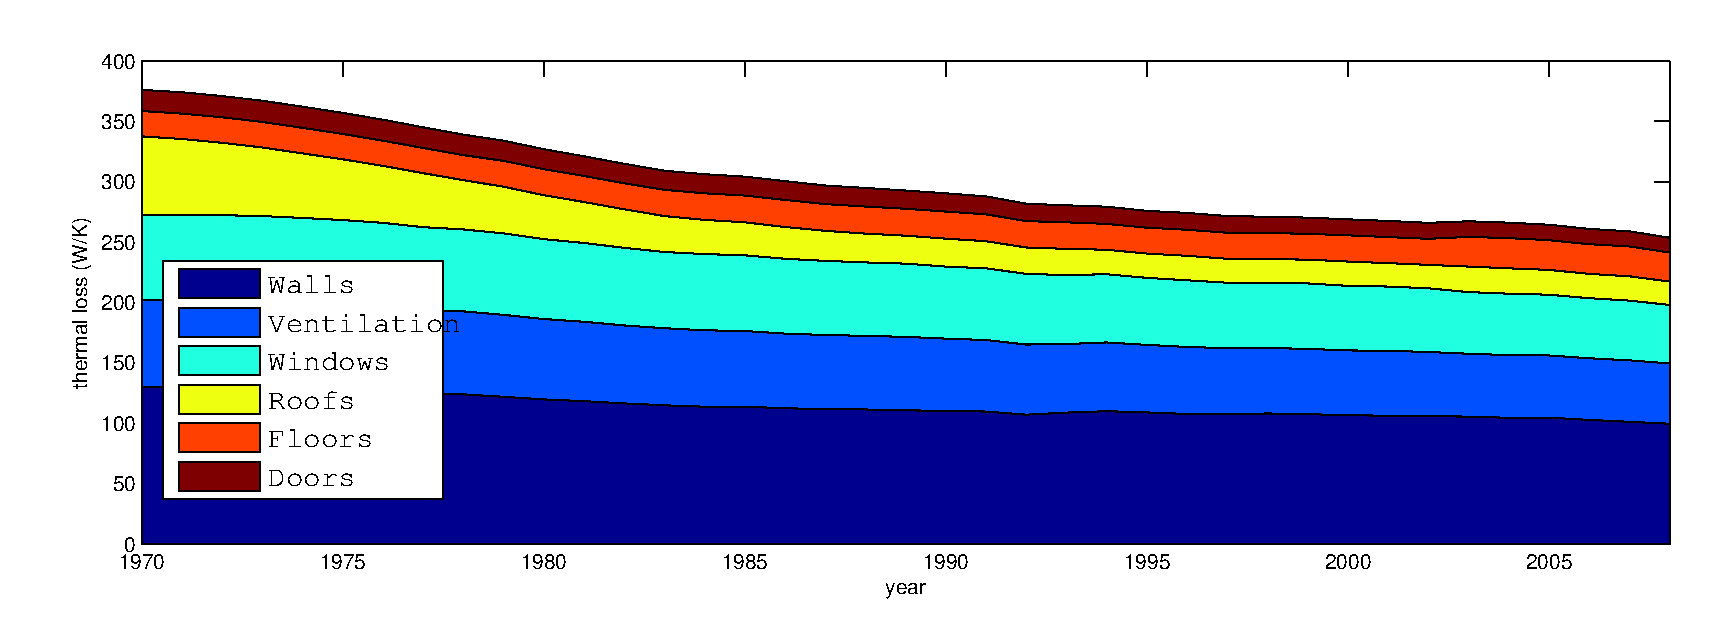
\includegraphics[width=0.8\textwidth]{images/house_insulation.eps}
\label{fig:houseins}
  \vspace{-10pt}
\end{figure}
\begin{figure}[h!]
  \vspace{-10pt}
  \caption{Year-on-year winter internal to external temperatures}
  \centering
    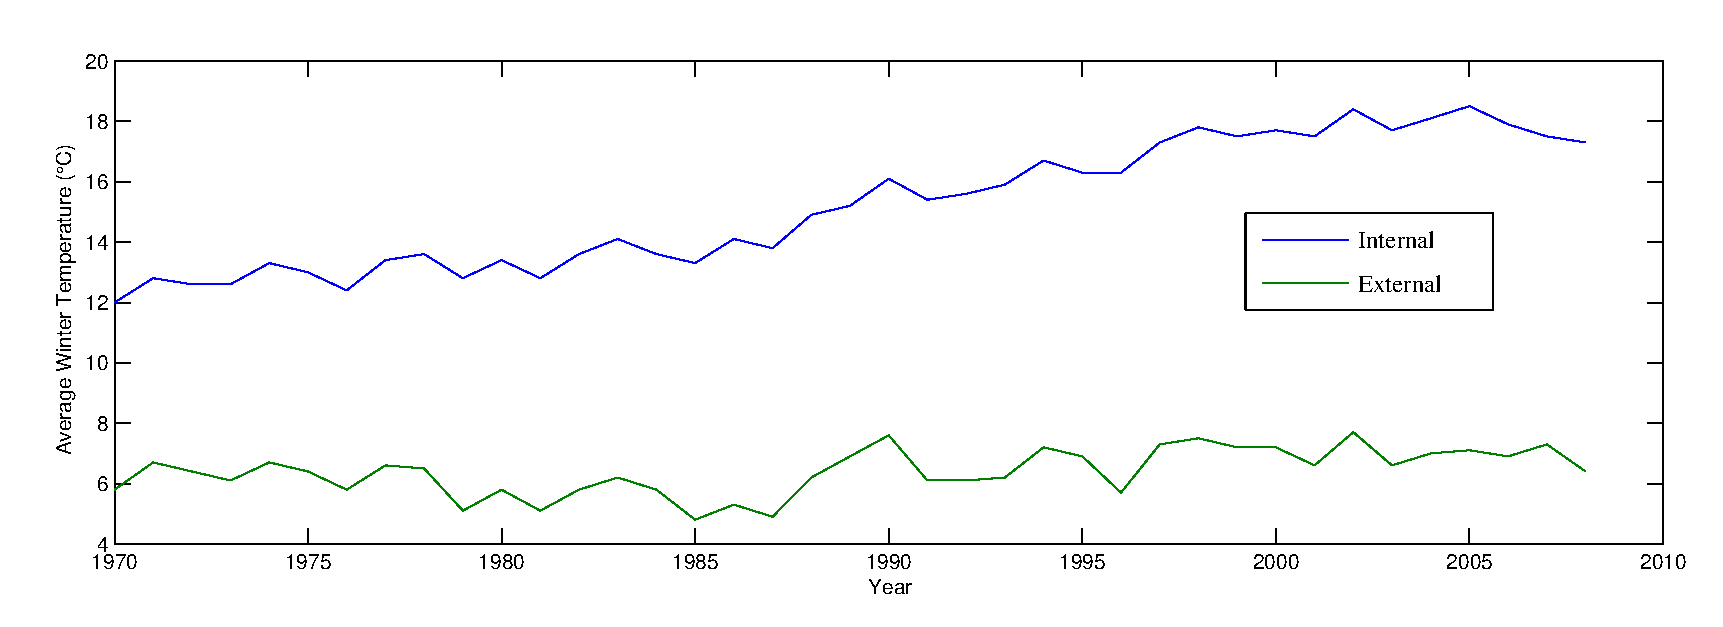
\includegraphics[width=0.8\textwidth]{images/winter_temperatures.eps}
\label{fig:housetempswint}
  \vspace{-10pt}
\end{figure}
\FloatBarrier
From this data, an estimation of the power usage can be made from the average winter temperature difference between inside and out. Taking data from 2008, the average temperature difference was 10.9 \celsius. With a thermal loss of 253.7 W/K, this means a power of 2.77 kW is required to heat the average home. The weighted average fuel price is 6.02p/kWh: meaning it costs 16.7 pence for every hour the central heating is switched on. Assuming that the heating is used for 12 hours a day, this means a daily cost of  \textsterling 2. Considering that the weekly expenditure on lights, heating and power is  \textsterling 18.90, this seems to be a reasonable estimate.

\begin{table}[h!]
    \begin{tabular}{|l|l|}
    \hline
    \textbf{System prediction benefit} & \textbf{Approximate hourly saving(\pounds)} \\ \hline
    Turning down temperature in sleep state     & 1.53 p/K                  \\ \hline
    Turn off heating whilst house is unoccupied & 16.7 p                    \\ \hline
    \end{tabular}
\end{table}

Above are the approximate hourly savings the home automation system can provide the average UK household during winter months per hour. Although these appear small, if the heating was turned down for 7 hours a day by 2 \celsius whilst the occupants are sleeping, and 1 hour or so of unnecessary heating is reduced every day, then the daily saving the system would provide will be around \pounds 0.40. This is a reduction in 20\%, which over the course of a year could be \pounds 130 for the average UK gas bill of \pounds 653 on direct debit.

Another way of estimating the amount the system could save is by thermally modelling a house and calculating the energy used for different thermostat settings: one set like a traditional thermostat, which maintains a temperature for 12 hours a day through the week and the entirety of Sunday; and one using simulated occupation data, which a machine learning algorithm could hopefully predict.

Fortunately, MATLAB has a Simulink model for a house heating system, so making the simulations was reasonably straightforward. The program was modified by firstly matching the program parameters to the thermal resistance, temperature and average p/kWh of a UK home as specified above. Additionally, the constant thermostat setting was replaced by a switchable signal generator giving either the AutoHome or conventional thermostat settings. The schematic for this model is shown in Figure \ref{fig:housesimu}.
\begin{figure}[h!]
  \vspace{-10pt}
  \caption{The House Heating Simulink Model}
  \centering
    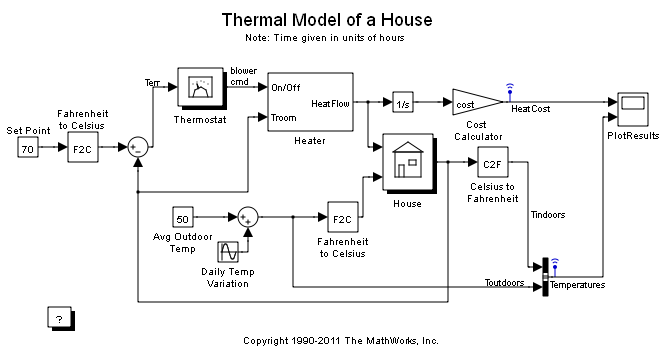
\includegraphics[width=0.8\textwidth]{images/matlabhouseheat.png}
\label{fig:housesimu}
  \vspace{-10pt}
\end{figure}
\FloatBarrier
The model works by switching on/off a "blower", which heats 1 kg of air every second to 50 \celsius when the internal temperature of the house deviates from the setpoint by more than 0.5 \celsius. A feedback loop inside the house block takes the thermal losses from the temperature gradient into account. Integrating the thermal power going into the house gives the energy used, which the cost can be calculated from. A weeks worth of thermostat settings (168 hours) is fed into the system for the conventional and occupancy setpoints, and the results shown in the graphs below. The external temperature, shown as green in the lower plots, oscillates sinusoidally with an amplitude of 4 \celsius\ around the average winter temperature in 2008 of 6.4 \celsius. 
\begin{figure}[h!]
  \vspace{-10pt}
  \caption{Simulation result for a week's worth of conventional thermostat program  heating cost and temperatures}
  \centering
    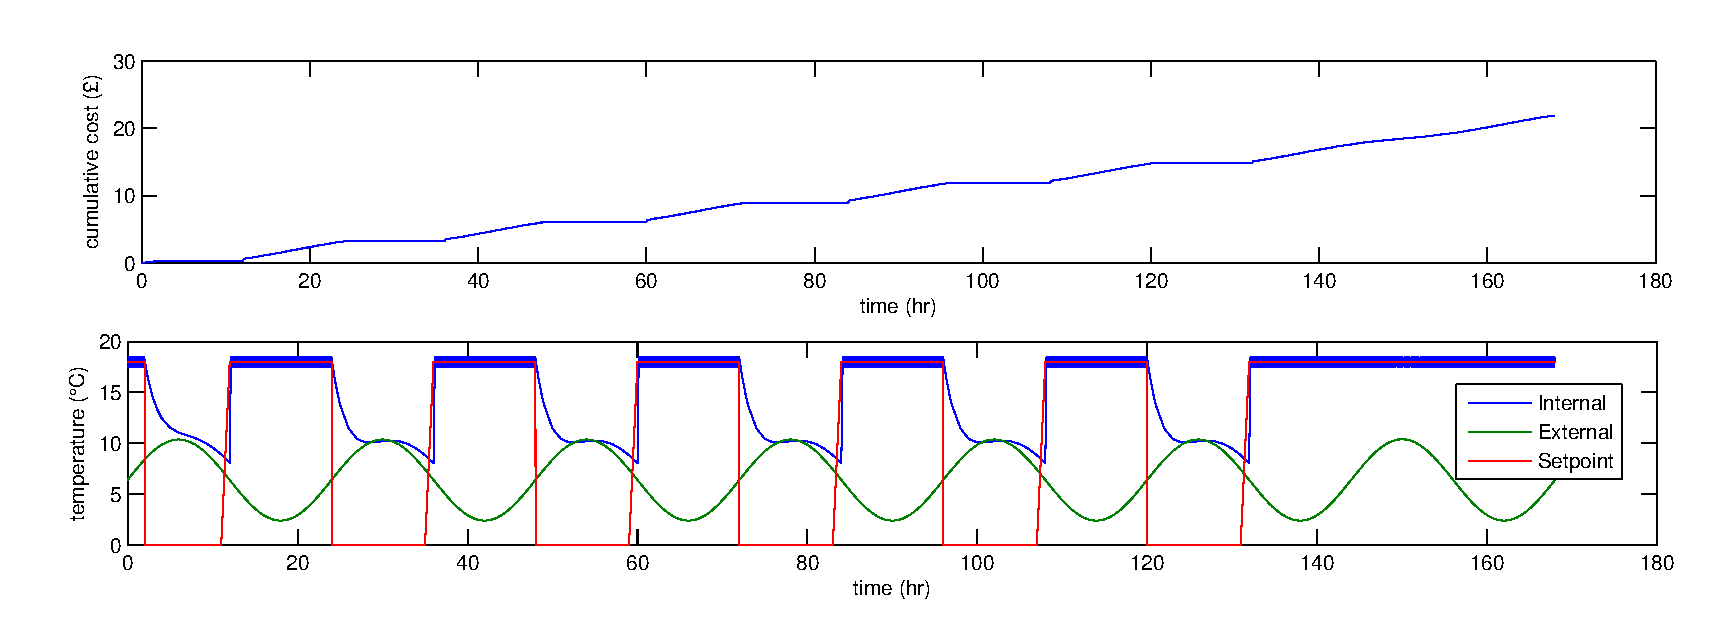
\includegraphics[width=0.8\textwidth]{images/thermal_m_conventional.eps}
\label{fig:convsimu}
  \vspace{-10pt}
\end{figure}
\begin{figure}[h!]
  \vspace{-10pt}
  \caption{Simulation result for a week's worth of predicted occupancy and corresponding thermostat setting  cost and temperatures}
  \centering
    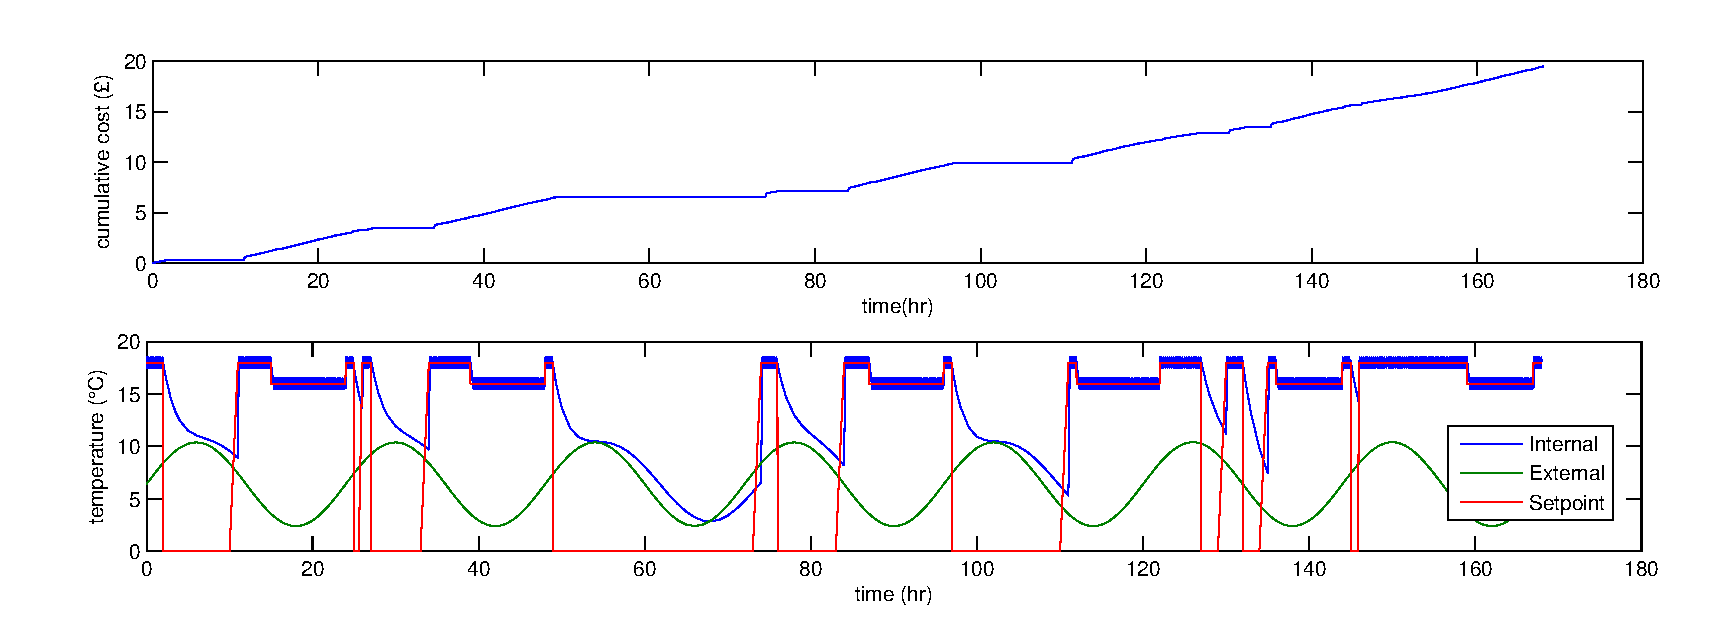
\includegraphics[width=0.8\textwidth]{images/thermal_m_autohome.eps}
\label{fig:autohsimu}
  \vspace{-10pt}
\end{figure}

The first thing to note is that the estimated costs are in the same ballpark of those predicted by simple calculation earlier at \pounds 21.90 and \pounds 19.48 respectively, which represents a saving of almost \pounds 2.50. Although this a quite a modest saving, it is worth revisiting the other aim of the automation system, which is to increase the comfort and convenience of the house's heating. Clearly the occupancy of the house is non uniform unlike the setting of the conventional system, which means there will be times when the house is either unnecessarily heated or at an uncomfortable temperature. 
\section{Hardware Performance}
Each module of the hardware was first developed separately and tested so in order tp fix any issues at their earliest stage. These were then all connected and the programmes combined to form a singular master programme which would control the whole mbed system.

First the digital temperature sensor was set up and programmed as discussed in section \ref{sec:sensors} after which initial tests found the temperature to be very low, however with the addition of pull-up resistors on the SCL and SDA pins the temperature was found to be as expected, this was then tested using an advanced handheld temperature sensor and was found to be accurate to $\pm$0.5\celsius\ as expected.

With the temperature sensor now completed the humidity sensor could be utilised, as it requires the local temperature in order to calculate the correct humidity from the input voltage which is measured using an ADC port on the mbed. This was then tested by measuring the outside environment with the humidity returned from the weather API, this was found to return similar values though the humidity sensor itself was not particularly stable and varied by several \% points. However this would be as expected as the datasheet tells us the $\pm$3\%.

With the local system complete, the wifly module was set up and connected to an access point setup using a laptop (as it cannot connect to enterprise enabled wifi). It was also tested using a standard home router which was supplied by the ISP company. After which a websocket connection was set up, this was generally successful but ran into a number of problems.

The first and major problem was that the websocket would close after an unknown period of time for unknown reasons. Furthermore the \verb+is_connected+ function failed to report when the websocket would disconnect, the general solution came from the common ping-pong idea. Where a ping was regularly sent from the mbed and the server would then return pong, if this return ‘pong’ was not detected by the mbed mode it would then re-join the websocket, however this was only partially successful and sometimes failed completely, and so a reset then reboot command was sent to the wifly module after which it would then reconnect quickly with no failures.


\section{Software Performance}
\subsection{Timetable Prediction}
Every three hours\footnote{This value can be changed but was chosen to be three hours as the algorithm works best by regressing on 6 hours of past data - however to accommodate for unexpected events and offer more granularity 3 hours was chosen as a good compromise} the timetable prediction program(described in section \ref{sec:ttpredictprog}) is called to predict what it expects the current day to look like, as well as what it expects (though with lower confidence) the other days of the week.  This is shown in Figure \ref{fig:ttblweb} which shows that the user is allowed to override the estimated timetable for advanced energy savings - however  as current systems work purely by such scheduling and are often seen as inefficient this use is discouraged.

This timetable is used if the current state is either \verb+away+ or \verb+asleep+ and is expected to be \verb+inside+ (which also implies awake) in the next 15 minutes\footnote{The certainty - i.e. if the algorithm is 50\% sure or 75\% sure - can be changed but is set to 50 by default}. When this is the case the house is heated up to the expected comfortable temperature (determined by the algorithm in section \ref{sec:gprmltemp}). It will sometimes be the case that the user does not come back when expected. In such a case a half-hour window will be given for the house state to become \verb+inside+ (i.e. detect someone is present) before ignoring this timetable and instead waiting for the house state to actually become \verb+inside+ to avoid energy waste (at the expense of compromising user comfort).

Testing the real world use of the predictor was a challenge as a lot of data would need to be collected - a feat not possible in the amount of time given. Instead the UMass SMART* dataset\cite{umasssmart} was used to test this data and determine the accuracy (which also allowed for finding the best parameters) as seen in Figure \ref{fig:predcons}. From this we can see that the expected accuracy is 85\% which is a reasonably good performance which however requires a fallback \& override in case of failure - which is described above.
\begin{figure}[h!]
  \vspace{-10pt}
  \caption{Timetable presented on website}
\textbf{Legend}:\\ \textcolor{red}{Red}: Asleep - \textcolor{green}{Green}: Inside - \textcolor{blue}{Blue}: Away\\
Dark: Algorithm Predicted State - \textcolor{dark-gray}{Light}: User Set State

  \centering
    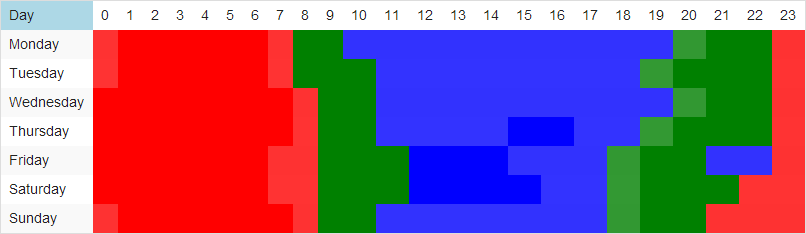
\includegraphics[width=1\textwidth]{images/ttble.png}
\label{fig:ttblweb}
  \vspace{-10pt}
\end{figure}
\FloatBarrier
\subsection{Website Usage}
The website was primarily tested in college using Google Chrome. This is because the site is only accessible internally to college (although it can be connect to elsewhere using the VPN) and Chrome is the only browser on the college computers that is up to date. Using a recent browser is important to the website, as it has regular use of websockets; a protocol only introduced in HTML5, along with a few other features not supported in older browsers. Unfortunately the other browsers on campus are not up to date enough to support websockets.

The first test for each page was to simply check for errors in the console window and address any issues that arose. After this, any major change made to the website was heavily tested for bugs by a handful of people. Any changes that were needed were made, with this process being repeated again for the updated version. The websockets could be tested easily by checking the websocket server log for messages, with the results of anything returned being displayed directly on the website.

Ajax requests could be checked in one of two ways. Firstly it can be checked that they are actually called and receive a response by using the network console window. This lets you see detailed information about any request, such as what data is sent with the request and any data that is returned. Secondly, because the ajax requests all deal with database handling, it is possible to check the relevant tables using mysql directly.

It is possible to check that the weather API script is collecting data correctly by viewing the graphs on the statistics page.

Once the website was fully functional in Chrome, it was also tested in latest versions of Internet Explorer and Firefox. A few small modifications were needed to ensure cross browser compatibility which were easily made. The site was also tested on IE9 mobile, where it failed due to lack of support for websockets, but was otherwise fine and also on safari for iOS, where it worked fully. The site is not however optimised for mobile use, this is where a phone app would come in use.
\section{System Practicality}
The practicality of the system was determined by assessing the ease at which it could be installed into a house. It is important the the entire system can be easily retro fitted to a house. Otherwise, only the relatively small number of new builds could get the benefits the system has to offer, which would render it both economically invalid and removes any real potential to impact the national or worldwide energy consumption. For each of the hardware modules, important considerations are how the component will be installed, maintained, the intrusion caused to the users and the security of it.     

The majority of UK households have a gas fired boiler, which is controlled by either bimetallic coil switch in mechanical thermostats or a relay in programmable flavours. For these, only four wires are needed: live, neutral and the two switch wires for the relay. Connecting the main mbed module to this can either be done directly or with a separate boiler relay unit included connected to the wireless ZigBee network. The thermostat then maintains the temperature at a given setpoint by switching on/off this relay. Whether the house has an oil, electric or gas boiler or a ground source heat pump, the thermostat can control a local temperature with ignorance. Installing such a system will be identical to any commercial programmable thermostat, which can be done by any plumber or even by the homeowner with relative ease.

Similarly, with the light switches, the electronics is simple enough to be integrated into a conventional light switch housing, and can be replaced easily. The power supply can be derived off the mains that it is switching. Furthermore, since the lightswitch is effectively just a wirelessly controllable mains supply with a bulb attached to it, the design can be used in any domestic appliance and embedded into a traditional mains socket or integrated into the appliance itself.

As for the power meter, the same current clip design is used in many of the commercially available ‘smart meters’ that are designed for the user to simply install themselves due to the safety of not having to touch the mains at any point. Although not implemented on the prototype, a very simple and sensible way to power to unit is through the voltage sense transformer by rectifying, smoothing and applying to the regulation circuit.

Motion sensors need to be in critical places such as main living spaces such as kitchen, bathroom and lounges, but also in bedrooms to determine sleep state. Naturally, the idea of having a wirelessly transmitting motion sensor especially in a bedroom may seem like an invasion of privacy, in reality they are only a passive infrared receiver with a digital output giving a change in radiation due to motion. Therefore, no information apart from the activity of the house, which is what the system is trying to ascertain, can be extrapolated. 
\section{System Unit Cost}
\textit{Note}: A breakdown of costs can be found in the appendix section \ref{sec:costs}.

As can be seen in the table above the final cost of the prototype came to \pounds 212.34 (including breadboard) . While this is above our expected costs this does not take into account any benefits from economies of scale, plus the advantages from component switching when working on PCB (as opposed to breakout boards required for breadboard). Furthermore the mbed development board is the most expensive unit for our prototype, however when finally developed only the microprocessor (and some other debugging components) will be required. This would drop the cost of the microprocessor from \pounds 41.38 to just \pounds 5.51 (for a single unit, lower for multiples) and so already it can be seen that there is significant scope for reductions before the final design.
\chapter{Further Development}
There are many ways in which this system could be enhanced, for example adding cameras or microphones to increase the detection rate of human presence. However many of these come at the cost of overcomplicating the device (and its installation) - for example the proposition of adding a camera not only complicates the installation and adds little benefits but also introduces privacy problems (many people would object to the installation of a camera in their home) - ultimately causing the product to be less attractive. Thus further developments must take this into account to genuinely improve the product and make it more attractive and useful rather than loading it with features.
\section{LCD Screen}
\section{Modular Network Setup}
One major improvement to our design would be the addition of a simple, ease of use module setup feature. This would be where different components could be purchased separately by the consumer and then with a simple few button touches would be connected into the network as a fully functional device, this could be done by using some of the abilities of Xbees which allows new Xbees to be easily included into a new network using an API framework.
\section{Smart Door Lock} 
This improvement would involve offering a module which can be installed on the main door of the house and compliment a usual key lock by offering a wireless solution. The advantages of such a lock would be the ability to open the main door simply via a digital key adding more possibilities for key control. For example the keys could be given to guests temporarily or only work for the cleaning lady at certain times and deactivated remotely. Digital security would evidently be a high priority of such a device. 

Additionally this type of device, while very new, is not innovative in itself as there are already two companies trying to enter this market - \href{http://lockitron.com}{Lockitron} and \href{http://www.august.com}{August Lock}. The real interest in offering this as a module would be near 95-99\% certainty in house occupancy\footnote{Assuming no pets which is another issue to deal with}. Indeed by combining the house motion sensors with main door traffic flow (which can be determined whether someone has just entered the house or not). The state can be determined by a process similar to:
\begin{itemize}
\item \textbf{Key used to enter house}: Assume someone is entering house thus presence is inferred
\item \textbf{Key not used}: Assume that someone is either leaving the house or guests are being let in. Differentiate by:
\subitem \textit{No motion detected in house up to 5 minutes after event}: Assume house empty (otherwise motion would be detected when moving inside house)
\subitem \textit{Motion detected 5 minutes after event}: Infer presence in house
\end{itemize}

While a Hidden Markov Model will still need to be relied upon to clearly differentiate states this method is expected to greatly increase house estimation accuracy while adding a useful module to the system.
\chapter{Conclusion}

\bibliographystyle{plain}
\begin{thebibliography}{1}
\bibitem{GBFactFile} Jason Palmer, Ian Cooper {\em Great Britain's Housing Energy Fact File} \url{https://www.gov.uk/government/uploads/system/uploads/attachment_data/file/48195/3224-great-britains-housing-energy-fact-file-2011.pdf}

\bibitem{DOE2008} L.D.Shorrock, J.I.Utley {\em Domestic Energy Fact File 2008} \url{http://www.bre.co.uk/filelibrary/pdf/rpts/fact_file_2008.pdf} 2008.

\bibitem{DOEFP2013} DOE {\em Annual Report on Fuel Poverty Statistics 2013} \url{https://www.gov.uk/government/uploads/system/uploads/attachment_data/file/199833/Fuel_Poverty_Report_2013_FINALv2.pdf} 2013.

\bibitem{mandmhomeauto} MarketsandMarkets {\em Global Home Automation \& Control Systems Market is expected to reach \$35,627.83 million by 2016}  \url{http://www.marketsandmarkets.com/PressReleases/home-automation-control-systems.asp} September 2011.

\bibitem{mandmiot} MarketsandMarkets {\em Internet of Things (IoT) \& Machine-To-Machine (M2M) Communication Market}  \url{http://www.marketsandmarkets.com/Market-Reports/internet-of-things-market-573.html} September 2012.

\bibitem{farnellnxplpc} Farnell UK {\em NXP - LPC1768FBD100 - MCU, 32BIT, ARM CORTEX M3, 100LQFP}  \url{http://uk.farnell.com/nxp/lpc1768fbd100/mcu-32bit-arm-cortex-m3-100lqfp/dp/1718549MPKG} June 2013.

\bibitem{houzzelgan} Mike Elgan {\em 
Home Tech: There's an Easier, Affordable Future for Home Automation}  \url{http://www.houzz.com/ideabooks/4307872/list/Home-Tech--There-s-an-Easier--Affordable-Future-for-Home-Automation} September 2012.

\bibitem{hmgovenergy} HM Government {\em 
Helping households to cut their energy bills}  \url{https://www.gov.uk/government/policies/helping-households-to-cut-their-energy-bills} May 2013.

\bibitem{doecc} Department of Energy and Climate Change {\em 
Smart Metering Implementation Programme Consultation document}  \url{https://www.gov.uk/government/uploads/system/uploads/attachment_data/file/42953/6129-consultation-second-version-smets.pdf} August 2012.

\bibitem{hartgw} Hart, G. W. {\em 
Residential energy monitoring and computerized surveillance via utility power flows}  \url{http://ieeexplore.ieee.org/stamp/stamp.jsp?tp=&arnumber=31557} 1989.

\bibitem{umasssmart} Sean Barker, Aditya Mishra, David Irwin, Emmanuel Cecchet, and Prashant Shenoy {\em Smart*: An Open Data Set and Tools for Enabling Research in Sustainable Homes} \url{http://lass.cs.umass.edu/papers/pdf/sustkdd-smart.pdf}

\bibitem{DOElighting} Department of Energy {\em Energy Efficiency and Renewable Energy} \url{http://energy.gov/sites/prod/files/energy_savers.pdf} 2011.

\bibitem{tulumwsu} Washington State University {\em WSU CASAS Datasets} \url{http://ailab.wsu.edu/casas/datasets/index.html}

\bibitem{msftresearch} James Scott, A.J. Bernheim Brush, John Krumm, Brian Meyers, Mike Hazas, Steve Hodges, Nicolas Villar {\em PreHeat: Controlling Home Heating Using Occupancy Prediction} \url{http://research.microsoft.com/en-us/um/people/jckrumm/publications\%202011/preheat-ubicomp2011\%20-\%20distribute.pdf} September 2011.


\bibitem{MITGPRbook} Carl Edward Rasmussen and Christopher K. I. Williams {\em Gaussian Processes for Machine Learning} \url{http://www.gaussianprocess.org/gpml/chapters/} 2006.

\bibitem{StanfordStats} Jonathan Taylor {\em Statistics 191: Introduction to Applied Statistics} \url{http://www-stat.stanford.edu/~jtaylo/courses/stats191/notes/simple.pdf} January 2009.

\bibitem{GPMLDoc} Carl Edward Rasmussen, Hannes Nickisch {\em Documentation for GPML} \url{http://www.gaussianprocess.org/gpml/code/matlab/doc/} January 2013.

\bibitem{GPROpt} Manuel Blum, Martin Riedmiller {\em Optimization of Gaussian Process Hyperparameters using Rprop} \url{http://ml.informatik.uni-freiburg.de/_media/publications/blumesann2013.pdf} 2013.

\bibitem{UManMND} University of Manchester {\em Multivariate Normal Distribution} \url{http://www.maths.manchester.ac.uk/~mkt/MT3732\%20(MVA)/Notes/MVA_Section3.pdf} 2010.

\bibitem{scikitlearn} Pedregosa et al. {\em Scikit-learn: Machine Learning in Python: Gaussian Processes} \url{http://amueller.github.io/modules/gaussian_process.html} 2013.

\bibitem{camgpr} Christopher K. I. Williams, Carl Edward Rasmussen {\em Gaussian Processes for Regression} \url{http://mlg.eng.cam.ac.uk/pub/pdf/WilRas96.pdf} 1996.

\bibitem{edsnelgpr} Ed Snelson {\em Tutorial: Gaussian process models} \url{http://mlg.eng.cam.ac.uk/tutorials/06/es.pdf} October 2006.

\bibitem{dukegpr} David P. Williams {\em Assessing Approximations for Gaussian Process Classification} \url{http://people.ee.duke.edu/~lcarin/David1.27.06.pdf} January 2006.

\bibitem{mbeddatasheet} ARM NXP {\em 32-bit ARM Cortex-M3 microcontroller Rev. 9 — 10 August 2012 Product data sheet} \url{http://www.nxp.com/documents/data_sheet/LPC1769_68_67_66_65_64_63.pdf} August 2012.

\bibitem{homewifi} Strategy Analytics {\em A Quarter of Households Worldwide Now Have Wireless Home Networks} \url{http://www.strategyanalytics.com/default.aspx?mod=pressreleaseviewer&a0=5193} April 2012.

\end{thebibliography}

\chapter{Appendix}
\section{Hardware}
\subsection{mbed}
\subsubsection{Main Control Code}
\label{sec:wificonnect}
\lstinputlisting[language=C]{code/homeauto-main.cpp}
\lstinputlisting[language=C]{code/homeauto-header.h}
\lstinputlisting[language=C]{code/homeauto-functions.cpp}

\subsubsection{XBee}
\label{sec:xbee}
\textbf{API Framework}


\begin{figure}[h!]
  \vspace{-10pt}
  \caption{XBee and XBee PRO wireless specifications}
  \centering
    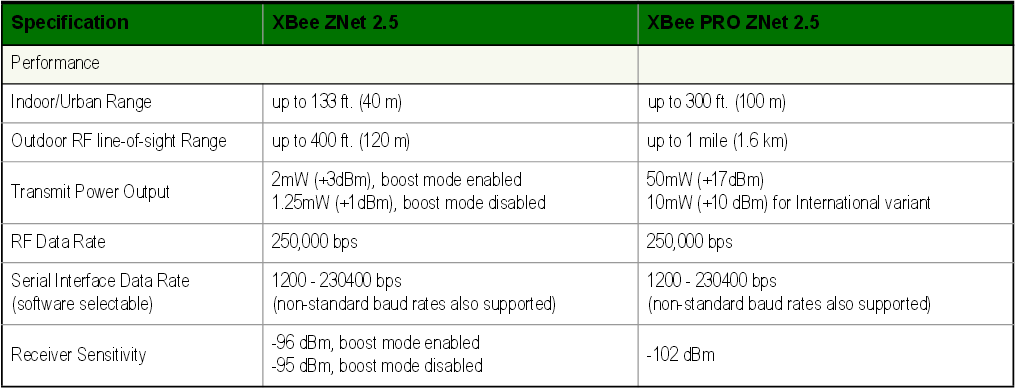
\includegraphics[width=1\textwidth]{images/xbeefig.png}
  \vspace{-10pt}
\end{figure}

The API framework consisted of 3 main sections. First is a function specific frame creator which allows an explicitly specified frame to be transmitted to the UART on the XBee. These frame creator functions are able to calculate their own checksums and account for different addresses as well. This allowed the specific frame requests to be transmitted at request. Next a function called \verb+readreply()+ was created in order to capture the reply from the XBees and store it in an array for that function. In most cases the reply came almost immediately, thus there was no need to wait at all for the reply. There are different variants of readreply which show the reply bytes if needed. Last is the \verb+readpacket()+ function which decoded the reply depending on what it is a reply to. This was achieved by scanning the incoming data and picking out a packet from the reply then looking at the frame specifier type which allowed us to see what kind of response it was. Once this had been done, it was possible to then decode the data from those packets in each case. As mentioned earlier the analogue reading which is a remote AT IS command response has 2 frame ids returned depending on which function created it.
Sensor Interfaces.

Our sensors use a variety of these features. 

The Motion sensors use the analogue inputs. The API frame for measuring the value on the ADC inputs is sent in the \verb+SENDSENSORREQ()+ function. This function also reads the reply and decodes the appropriate bits to get the analogue value back. The ADC input only goes from 0 to 1.2V though so the levels it can read are different from the motion sensor output which is VDD-0.5 where VDD is 3.3V. Thus we used a potential divider to scale the voltage down around 0.8V for motion and 0.5V for no motion. This allows us to see when motion has been detected.

\textbf{Light}

In order to control the light switches with the XBee, we had to implement extra digital logic. This was controlled from two sides, where the physical light switch was one and the digital output from the XBee was the other. In order to service the web socket requests the digital IO functions for the XBee were called by using either \verb+SENDLIGHTONREQ()+ or \verb+SENDLIGHTOFFREQ()+. These functions either pulled the pin high or low depending on which one was called. This gave the other input to the XOR gate which allows the triac circuit to turn the light on or off accordingly. The other job the XBee has is to measure the current output of the XOR gate in order to get the current status of the light. This is needed in order to update the graphic on the website relating to the relevant light toggle switch. In the end two ways were attempted to accomplish this. 

The first was a polling based method which we ended up using; this method uses a similar analogue function as the motion sensor readings used. This was done in order to save a bit of time when writing the code, as the speed of detection was not an issue. When the function \verb+SENDLIGHTSTATUS()+ is called the XBee calls for an analogue reading which is a scaled down version of the digital level on the XOR gate. As well as giving an analogue reading a different frame ID is returned in order to differentiate between motion sensor readings and light switch readings. These are then loaded into global variables and passed via web socket.
Our second method was to use UART interrupts along with the XBee pin change detection feature. The XBee can detect rising and falling edges on its monitored digital inputs. When an edge occurs the corresponding API frame is transmitted. The interrupts on the UART allow the MBED to listen for this reply which could come in at any time. Unfortunately the result turned out to be buggy as the modified serial library with a circular buffer had strange behaviour. getc() would not read the characters in the correct order, whilst using a function called \verb+rxGetLastChar()+ the operation worked fine until the buffer filled up. After flushing this buffer the UART only read in 5 or 6 bytes at a time.
The standard serial library worked fine with the interrupts on the UART however not all of the XBee frames can be captured correctly as there is only a 16 byte buffer on the FIFO. Thus this idea was not used in the end. Since we chose to go down the polling route, there is a 3 second lag on how long it takes for the graphic on the webpage to update.

\textbf{Power}

The power sensor interfaced slightly differently to the other sensors. As there is a ATmega microcontroller on the sensor circuit it was decided that transferring the data as 16 bit short integers over UART would be most efficient. This was the case as the ADCs in the XBee are only 10 bit and would introduce more error into the measurements. Due to the serial interrupts not working as expected a workaround was devised, as it was not possible to just send a raw UART frame we leveraged the ATmega controller to help us. The power readings are taken on a regular poll using a standard timer in the MBED like every other function. When this timer activates the digital output on the power XBee is pulled high. This  causes an interrupt to occur on the rising edge of the signal which causes the ATmega controller to explicitly send a new API frame containing raw data with the numbers to the co-ordinator XBee. A small wait happens in between these two functions in order to make sure that the circular buffer is filled with the UART data. After receiving and decoding the data, a request to set the XBee digital pin low is sent, and the sensor will be ready for another reading the next time \verb+SENDPOWERREQ()+ is called.

\textbf{Issues with interrupts}

At the beginning the ideal vision of how we would have handled XBee communication would have been to use ISRs to service requests as needed. For simplicities sake due to timing we decided that a polling based method would be more robust and just as viable. In order to use an interrupt based approach we would have to have had full interrupt capability on all of the UART ports so that ISRs could be activated upon the required JSON strings entering the system. Taking a poll based approach we used the timers on the Cortex-M3 in order to activate interrupts at specified time intervals. One problem with this was the fact that whilst one ISR was running, it could not be interrupted at all, so nested interrupts were not possible with this approach. If the ISR was interrupted again whilst sending out an API frame to the UART it would simply be discarded as invalid data. If an interrupt occured when the XBee received a frame, that data would then have been missed as well and the whole thing would have had to have been done again. Thus all interrupts were disabled globally for the duration of the XBee ISRs. This was done with the function calls \verb+__disable_irq()+ and \verb+__enable_irq+. This ultimately limits the amount of processing that can occur on the CPU core as the ISRs are effectively blocking functions, and thus nothing else can run whilst they do. In the case of the power routine, there is a 200ms wait in there which squanders a lot of cycles however it has to be there in order to capture the response, thus in this instance an interruptable UART would have been superior. With polling comes inevitable latency between polls as well which can be several seconds. This is most noticeable when polling for the light context at which point the true context isn't updated for up to 3 seconds if the most recent poll has just passed. This causes a slight glitchyness on the web interface, however after the next poll it would correct itself.

\textbf{Code}
\lstinputlisting[language=C]{code/homeauto-xbeeC.cpp}
\lstinputlisting[language=C]{code/homeauto-xbee.h}
\subsection{Wireless Power Monitoring}
\subsubsection{Power Diagram}
\begin{figure}[h!]
\centering
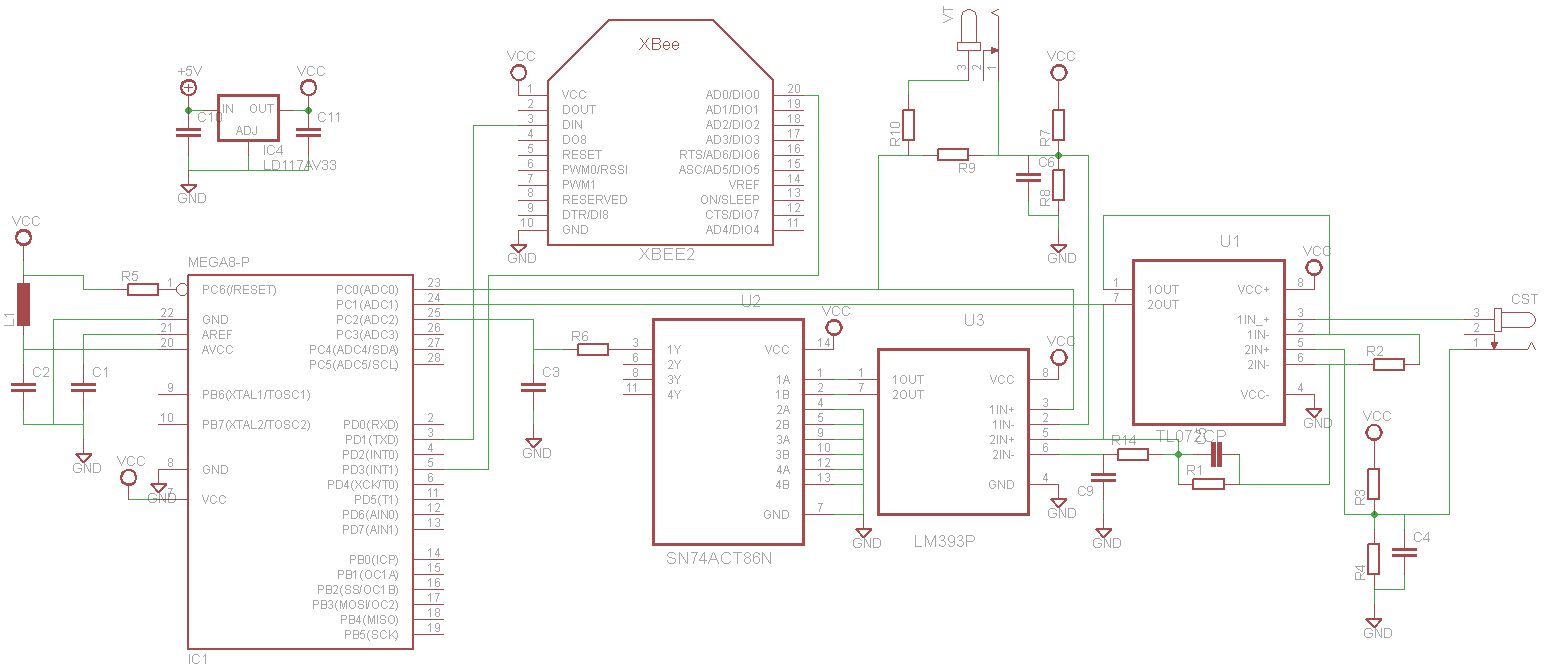
\includegraphics[width=1.5\textwidth, angle=90]{images/power_diagram.png}
\caption{Power meter circuit diagram}
\end{figure}
\section{Software}
\subsection{Server Code}
\label{sec:tornadocode}
\lstinputlisting[language=Python]{code/tornado_ws.py}
\subsection{Timetable Prediction}
\subsubsection{Choice of day}
\label{sec:daychoice}
\begin{alltt}
\underline{\textbf{Testing how many days to take the mode}}
Obtained from: University of Massachusetts Amherst SMART* dataset
\underline{Acc Avg}: Is the average accuracy as prediction algorithm is tested on a full 
3 months of data
\underline{Std.Dev.}: is the standard deviation in the average accuracy for each day
\underline{len}: is the number of days of which the mode is taken to predict the future
\underline{s_p}: number of past samples used to take the hamming distance of - for example 
144 samples corresponds to 12 hours when the sampling is 5 minutes (the case in this data)
\underline{s_f}: number of future samples taken to then check the 
accuracy against the know future data
Acc Avg:79.2% Std.Dev.:20% w/day len=2 s_p=144 s_f=144
Acc Avg:79.9% Std.Dev.:22% w/day len=3 s_p=144 s_f=144
\textbf{Acc Avg:81.5% Std.Dev.:21% w/day len=4 s_p=144 s_f=144}
Acc Avg:80.6% Std.Dev.:21% w/day len=5 s_p=144 s_f=144
Acc Avg:80.5% Std.Dev.:21% w/day len=6 s_p=144 s_f=144
Acc Avg:79.5% Std.Dev.:21% w/day len=7 s_p=144 s_f=144
Acc Avg:79.0% Std.Dev.:22% w/day len=8 s_p=144 s_f=144
Acc Avg:79.0% Std.Dev.:22% w/day len=9 s_p=144 s_f=144
Acc Avg:79.0% Std.Dev.:22% w/day len=10 s_p=144 s_f=144
Acc Avg:79.3% Std.Dev.:23% w/day len=11 s_p=144 s_f=144
Acc Avg:79.3% Std.Dev.:23% w/day len=12 s_p=144 s_f=144
Acc Avg:79.3% Std.Dev.:23% w/day len=13 s_p=144 s_f=144
Acc Avg:79.3% Std.Dev.:23% w/day len=14 s_p=144 s_f=144
Acc Avg:79.3% Std.Dev.:23% w/day len=15 s_p=144 s_f=144
Acc Avg:79.3% Std.Dev.:23% w/day len=16 s_p=144 s_f=144
Acc Avg:79.3% Std.Dev.:23% w/day len=17 s_p=144 s_f=144
Acc Avg:79.3% Std.Dev.:23% w/day len=18 s_p=144 s_f=144
Acc Avg:79.3% Std.Dev.:23% w/day len=19 s_p=144 s_f=144
Acc Avg:79.3% Std.Dev.:23% w/day len=20 s_p=144 s_f=144
Acc Avg:79.3% Std.Dev.:23% w/day len=21 s_p=144 s_f=144
Acc Avg:79.3% Std.Dev.:23% w/day len=22 s_p=144 s_f=144
Acc Avg:79.3% Std.Dev.:23% w/day len=23 s_p=144 s_f=144
Acc Avg:79.3% Std.Dev.:23% w/day len=24 s_p=144 s_f=144
Acc Avg:79.3% Std.Dev.:23% w/day len=25 s_p=144 s_f=144
Acc Avg:79.3% Std.Dev.:23% w/day len=26 s_p=144 s_f=144
Acc Avg:79.3% Std.Dev.:23% w/day len=27 s_p=144 s_f=144
Acc Avg:79.3% Std.Dev.:23% w/day len=28 s_p=144 s_f=144
Acc Avg:79.3% Std.Dev.:23% w/day len=29 s_p=144 s_f=144
Acc Avg:79.3% Std.Dev.:23% w/day len=30 s_p=144 s_f=144



Acc Avg:74.9% Std.Dev.:26% w/day len=2 s_p=144 s_f=72
Acc Avg:76.9% Std.Dev.:27% w/day len=3 s_p=144 s_f=72
\textbf{Acc Avg:80.1% Std.Dev.:27% w/day len=4 s_p=144 s_f=72}
Acc Avg:78.3% Std.Dev.:28% w/day len=5 s_p=144 s_f=72
Acc Avg:77.8% Std.Dev.:29% w/day len=6 s_p=144 s_f=72
Acc Avg:75.9% Std.Dev.:29% w/day len=7 s_p=144 s_f=72
Acc Avg:74.8% Std.Dev.:31% w/day len=8 s_p=144 s_f=72
Acc Avg:74.8% Std.Dev.:31% w/day len=9 s_p=144 s_f=72
Acc Avg:74.8% Std.Dev.:31% w/day len=10 s_p=144 s_f=72
Acc Avg:75.4% Std.Dev.:31% w/day len=11 s_p=144 s_f=72
Acc Avg:75.4% Std.Dev.:31% w/day len=12 s_p=144 s_f=72
Acc Avg:75.4% Std.Dev.:31% w/day len=13 s_p=144 s_f=72
Acc Avg:75.4% Std.Dev.:31% w/day len=14 s_p=144 s_f=72
Acc Avg:75.4% Std.Dev.:31% w/day len=15 s_p=144 s_f=72
Acc Avg:75.4% Std.Dev.:31% w/day len=16 s_p=144 s_f=72
Acc Avg:75.4% Std.Dev.:31% w/day len=17 s_p=144 s_f=72
Acc Avg:75.4% Std.Dev.:31% w/day len=18 s_p=144 s_f=72
Acc Avg:75.4% Std.Dev.:31% w/day len=19 s_p=144 s_f=72
Acc Avg:75.4% Std.Dev.:31% w/day len=20 s_p=144 s_f=72
Acc Avg:75.4% Std.Dev.:31% w/day len=21 s_p=144 s_f=72
Acc Avg:75.4% Std.Dev.:31% w/day len=22 s_p=144 s_f=72
Acc Avg:75.4% Std.Dev.:31% w/day len=23 s_p=144 s_f=72
Acc Avg:75.4% Std.Dev.:31% w/day len=24 s_p=144 s_f=72
Acc Avg:75.4% Std.Dev.:31% w/day len=25 s_p=144 s_f=72
Acc Avg:75.4% Std.Dev.:31% w/day len=26 s_p=144 s_f=72
Acc Avg:75.4% Std.Dev.:31% w/day len=27 s_p=144 s_f=72
Acc Avg:75.4% Std.Dev.:31% w/day len=28 s_p=144 s_f=72
Acc Avg:75.4% Std.Dev.:31% w/day len=29 s_p=144 s_f=72
Acc Avg:75.4% Std.Dev.:31% w/day len=30 s_p=144 s_f=72

Acc Avg:79.6% Std.Dev.:25% w/day len=2 s_p=144 s_f=36
Acc Avg:80.6% Std.Dev.:25% w/day len=3 s_p=144 s_f=36
\textbf{Acc Avg:84.0% Std.Dev.:25% w/day len=4 s_p=144 s_f=36}
Acc Avg:81.2% Std.Dev.:28% w/day len=5 s_p=144 s_f=36
Acc Avg:80.5% Std.Dev.:28% w/day len=6 s_p=144 s_f=36
Acc Avg:77.8% Std.Dev.:29% w/day len=7 s_p=144 s_f=36
Acc Avg:76.2% Std.Dev.:30% w/day len=8 s_p=144 s_f=36
Acc Avg:76.2% Std.Dev.:30% w/day len=9 s_p=144 s_f=36
Acc Avg:76.2% Std.Dev.:30% w/day len=10 s_p=144 s_f=36
Acc Avg:77.1% Std.Dev.:30% w/day len=11 s_p=144 s_f=36
Acc Avg:77.1% Std.Dev.:30% w/day len=12 s_p=144 s_f=36
Acc Avg:77.1% Std.Dev.:30% w/day len=13 s_p=144 s_f=36
Acc Avg:77.1% Std.Dev.:30% w/day len=14 s_p=144 s_f=36
Acc Avg:77.1% Std.Dev.:30% w/day len=15 s_p=144 s_f=36
Acc Avg:77.1% Std.Dev.:30% w/day len=16 s_p=144 s_f=36
Acc Avg:77.1% Std.Dev.:30% w/day len=17 s_p=144 s_f=36
Acc Avg:77.1% Std.Dev.:30% w/day len=18 s_p=144 s_f=36
Acc Avg:77.1% Std.Dev.:30% w/day len=19 s_p=144 s_f=36
Acc Avg:77.1% Std.Dev.:30% w/day len=20 s_p=144 s_f=36
Acc Avg:77.1% Std.Dev.:30% w/day len=21 s_p=144 s_f=36
Acc Avg:77.1% Std.Dev.:30% w/day len=22 s_p=144 s_f=36
Acc Avg:77.1% Std.Dev.:30% w/day len=23 s_p=144 s_f=36
Acc Avg:77.1% Std.Dev.:30% w/day len=24 s_p=144 s_f=36
Acc Avg:77.1% Std.Dev.:30% w/day len=25 s_p=144 s_f=36
Acc Avg:77.1% Std.Dev.:30% w/day len=26 s_p=144 s_f=36
Acc Avg:77.1% Std.Dev.:30% w/day len=27 s_p=144 s_f=36
Acc Avg:77.1% Std.Dev.:30% w/day len=28 s_p=144 s_f=36
Acc Avg:77.1% Std.Dev.:30% w/day len=29 s_p=144 s_f=36
Acc Avg:77.1% Std.Dev.:30% w/day len=30 s_p=144 s_f=36
\end{alltt}

\subsubsection{Matlab Timetable Prediction Test Script}
\label{sec:matlabttpredict}
\lstinputlisting[language=Matlab]{general_prediction.m}

\subsubsection{Python code to predict timetable}
\label{sec:py-sqlttpred}
\lstinputlisting[language=Python]{sql-ttfill.py}

\subsection{Gaussian Process Regression}

%start
\subsubsection{General Machine Learning (ML) Terminology}


\textbf{\textit{Features}} are the input variables to the algorithm, i.e. if the algorithm is the function that outputs thermostat settings\textbf{,} then the features of the ML algorithm are the inputs or the feature space/domain. Features are inputted as vectors typically denoted by$\ {\mathbf x}$. Our choice of features was dictated by what made logical sense by the data available to us. The features selected are listed below:
\begin{enumerate}
\item  External Temperature

\item  External Humidity

\item  Internal Humidity

\item  Wind Speed

\item  Wind Direction
\end{enumerate}

\noindent (Internal temperature was omitted as this would provide unwanted feedback on the feedback from the control system, which the thermostat uses to regulate the internal temperature)

\begin{enumerate}
\item  \textbf{\textit{Training data set - }}is the set of feature vectors or `training examples' in the feature space that the algorithm uses to fit its regression curve in order to predict the thermostat setting for different conditions.

\item  \textbf{\textit{Target data set -} }is the set of outputs (in this context thermostat settings) for each of the training data points. 

\item  \textbf{\textit{Model Parameters - }}are the set of unknown coefficients of the model that is applied to the data. Linear Regression is an example of a parametric approach in which a model is chosen and then the parameters of the model are optimized to best fit the data. 

\item  \textbf{\textit{Hyperparameters - }}are important in non- parametric models such as Gaussian Process Regression. Gaussian Process Regression has no direct parameters to find or optimize, but it does have parameters for the prior, i.e. the coefficients of the covariance function. These need to be optimized to fit the data in a similar way to model parameters in parametric regression. 

\item  \textbf{\textit{Hypothesis - }}also known as the regression curve is the function that is inferred from the training data.
\end{enumerate}


\subsubsection{Terms and Definitions for GPR:}

\begin{enumerate}
\item \textbf{\textit{Random Variable}} -- A random variable is a variable that can take on a set of possible values each with an associated probability. 

\item  \textbf{\textit{Prior Probability }}--the probability distribution that one assigns to a quantity that expresses the uncertainty about the process before any data is observed. In GPR we assume a Gaussian distribution prior.

\item  \textbf{\textit{Likelihood }}-- the probability of the system parameters given the data that is observed.

\item  \textbf{\textit{Marginal Likelihood }}--the likelihood function integrated over certain parameters. In this way the parameters have been `marginalized'. It is also known as the `model evidence' because integrating this over the function $f$   gives the probability of the data given the chosen hyperparameters. 

\item  \textbf{\textit{Posterior Probability }}--The conditional probability that is assigned once relevant data and information is taken into account. 

\item  \textbf{\textit{Covariance}} - A measure of how much two random variables change with one another. 

\item  \textbf{\textit{Stochastic Process}} -- is a collection of random variables. 

\item  \textbf{\textit{Covariance Function}} -- For a stochastic process or random field, a covariance function describes the spatial covariance of points in the random field located at certain points in space. Covariance functions belong to a family of mapping functions called `kernels'.  

\item  \textbf{\textit{Multivariate Gaussian distribution}} --a generalization of the standard Gaussian or Normal distribution to multiple dimensions. It is described by a mean vector with a separate mean for each dimension, and a covariance matrix (a generalization of variance to multiple dimensions). It gives a similarity measure of each point with every other point in the distribution and is expressed as:
\[{\mathbf \beta }\ \sim \ N({\mathbf \mu },\ {\mathbf K})\] 
\end{enumerate}
${\mathbf \beta }$\textbf{ }is a multi-dimensional random vector, ${\mathbf \mu }$ is a mean vector defining the mean for each dimension\textbf{, }and \textbf{K} is the covariance matrix, detailing how much each random variable of  ${\mathbf x}$ changes with another, defined as:
\[{\mathbf K}=\ \left[\left( \begin{array}{ccc}
k\left({{\mathbf x}}_{{\mathbf 1}},\ {{\mathbf x}}_{{\mathbf 1}}\right) & \cdots  & k\left({{\mathbf x}}_{{\mathbf 1}},\ {{\mathbf x}}_{{\mathbf n}}\right) \\ 
\vdots  & \ddots  & \vdots  \\ 
k\left({{\mathbf x}}_{{\mathbf n}},\ {{\mathbf x}}_{{\mathbf 1}}\right) & \cdots  & k\left({{\mathbf x}}_{{\mathbf n}},\ {{\mathbf x}}_{{\mathbf n}}\right) \end{array}
\right)\right]\] 

 The Probability Density Function (PDF) of a Multivariable Gaussian Distribution is:
\begin{equation}
pdf_{\beta }=P\left({\mathbf \beta }{\mathbf =}{\mathbf a}\right)={\left(2\pi \right)}^{-\left(\frac{n}{2}\right)}{\left|{\mathbf K}\right|}^{-0.5}\exp\left(-\frac{1}{2}{\left({\mathbf a}-{\mathbf \mu }\ \right)}^T{{\mathbf K}}^{-1}({\mathbf a}-{\mathbf \mu })\right)
\end{equation}
\begin{enumerate}
\item  \textbf{\textit{Gaussian Process}} -  Is a stochastic process whose random variables, associated with each point in the random domain space, have a normal distribution. A Gaussian process can be thought of/visualised as an infinite dimensional Gaussian distribution. It is defined as:
\[f\left({\mathbf x}\right)\ \sim \ GP(m({\mathbf x}),\ k\left({{\mathbf x}}_{{\mathbf i}}{\mathbf ,\ }{{\mathbf x}}_{{\mathbf j}}\right){\rm \ })\ \] 
\end{enumerate}
$m({\mathbf x})\ $ is the mean function and `$k\left({{\mathbf x}}_{{\mathbf i}}{\mathbf ,\ }{{\mathbf x}}_{{\mathbf j}}\right)$' is the similarity or covariance function that measures the similarity between two random variables of the Gaussian process. For ease of computation, and without loss of generality we can set $m\left(x\right)=0$ as summing an infinite array of possible functions averages to 0. An important property of a Gaussian Process is that it obeys the consistency requirement; i.e. inspection of a larger set of random variables does not change the distribution of a smaller set. Every finite collection of these random variables can be described with a multivariate Gaussian distribution. 


\subsubsection{Algorithms and their Complexity:}

\noindent For this system to operate effectively three algorithms/functions are required; one to search the error curve to find a range of hyperparameter initialisations that find an acceptable minima, a second to train the GPR and a third to run the GPR and return a predicted thermostat setting. In this section \textit{`m'} denotes the number of features and \textit{`n'} the number of examples in the training set. Furthermore n$>$$>$m,  n$>$$>$ any loop counters

\noindent \textbf{\textit{Algorithm 1: Hyperparameter Search}}

\noindent Description:

\noindent Called every time a significant change in the training data is detected, so fairly infrequently (e.g. the first time the training data reaches its maximum capacity, or when a significant amount of data is changed).

\noindent \textbf{Pseudo code:}

\begin{enumerate}
\item \textbf{ }Import training data into \textbf{X} and cross validation data into ${{\mathbf x}}^{{\mathbf *}}$\textbf{ }

\item  Define upper and lower bound (ub and lb) as the boundaries within which to initialise ${\mathbf \theta }$ values. Initialise over some very large range. 

\item  Grid Search:
\end{enumerate}

\noindent while (ub -- lb)$>$1
\[{\rm \ \ \ \ \ \ \ \ \ \ \ \ \ \ \ increment\ =(ub-lb)}{\rm /numb\_div}\] 
lb\_temp = lb

 for j = 1-$>$(numb\_div -- 1)

  Initialise ${\mathbf \theta }$\textbf{ }in range(lb\_temp, ub)

  Train the GPR

  Run the cross validation data through `GPR Run' 
\[{\rm AvError[j]}=\frac{1}{n}\ \sum^n_{i=1}{\left\{\frac{\left(y_i-ypred_i\right)*100}{y_i}\right\}}\] 

 minIndex =  index of minimum element in ${\rm AvError[j]}$

 ub = lb +minIndex*increment

 lb = lb + (minIndex-1)*increment

\begin{enumerate}
\item  Write upper bound and lower bound values to SQL database to be used by `GPR train'
\[[Total\ Complexity\ \approx \ {{\log }_{numb_{div}} \left(ub-lb\right)\ }*nu{mb}_{div}*\left(O\left(n\right)+O\left(n^2\right)+O\left(n^3\right)\right)\approx O\left(n^3\right)]\] 
\end{enumerate}
\textbf{\textit{Algorithm 2: GPR Train}}

\noindent \textbf{Description:}

\noindent Called every time the training data set is updated. Calculates the inverse covariance matrix (plus noise) and the optimized hyperparameters, which are then both written back to the SQL database to be used by the `GPR run' algorithm.  As an aside the complexity of the kernel $k\left({{\mathbf x}}_{{\mathbf n}},\ {{\mathbf x}}_{{\mathbf n}}\right)$ is, considering only multiplications, divisions, subtractions and additions, $\left(m^2+m+1\right)\approx O(m^2)$

\noindent \textbf{Pseudo code:}

\begin{enumerate}
\item \textbf{ }Import training data from SQL database into \textbf{X} and the target data into \textbf{y}

\item  Normalize \textbf{X}: $\forall x_i\ in\ {\mathbf X}{\mathbf ,\ }x_i=\ \frac{{(x}_i-\mu )}{{\sigma }_n}$  (his ensures that all features are equally important and improves performance for gradient descent as each dimension has a similar range of relevant magnitudes) 

\item  Initialise hyperparameters, ${\mathbf \theta }$, by taking values from a uniform distribution with limits found by the hyper parameter search

\item  Gradient Descent:
\end{enumerate}

\noindent for j = 1-$>$max\_iters \textbf{or} until $L\left(\theta \right)$ not decreasing \textbf{or }$L\left(\theta \right)<desired\_error$
\[\ \ \ \ \ \ \ \ \ \ \ \ \ \ \ \ {\mathbf C}=\ \left[\left( \begin{array}{ccc}
k\left({{\mathbf x}}_{{\mathbf 1}},\ {{\mathbf x}}_{{\mathbf 1}}\right){+\sigma }^2_n{{\mathbf \delta }}_{{\mathbf ij}}\  & \cdots  & k\left({{\mathbf x}}_{{\mathbf 1}},\ {{\mathbf x}}_{{\mathbf n}}\right){+\sigma }^2_n{{\mathbf \delta }}_{{\mathbf ij}} \\ 
\vdots  & \ddots  & \vdots  \\ 
k\left({{\mathbf x}}_{{\mathbf n}},\ {{\mathbf x}}_{{\mathbf 1}}\right){+\sigma }^2_n{{\mathbf \delta }}_{{\mathbf ij}} & \cdots  & k\left({{\mathbf x}}_{{\mathbf n}},\ {{\mathbf x}}_{{\mathbf n}}\right){+\sigma }^2_n{{\mathbf \delta }}_{{\mathbf ij}} \end{array}
\right)\right] [n^2\left(2m^2+1\right)\approx O\left({n^2m}^2\right)]\] 
\[L({\mathbf \theta })=\ \frac{1}{2}y^TC^{-1}y+\frac{1}{2}{\log  \left(\left|C\right|\right)\ }+\left(\frac{n}{2}\right){\log  \left(2\pi \right)\ } [O\left(n^2\right)+O\left(n^3\right)\approx O\left(n^3\right)]\] 


  for i = 1-$>$ numb\_hyperparameters
\[{\theta }_i={\theta }_i-\ \alpha \frac{\partial L\left({\mathbf \theta }\right)}{\partial {\theta }_i} [n^3+2n+2n^2\approx O\left(n^3\right)]\] 

Return ${\mathbf \theta }$\textbf{}

\begin{enumerate}
\item \textbf{ }Using optimized ${\mathbf \theta }$ values calculate ${\mathbf C}=\ \left[\left( \begin{array}{ccc}
k\left({{\mathbf x}}_{{\mathbf 1}},\ {{\mathbf x}}_{{\mathbf 1}}\right){+\sigma }^2_n{{\mathbf \delta }}_{{\mathbf ij}}\  & \cdots  & k\left({{\mathbf x}}_{{\mathbf 1}},\ {{\mathbf x}}_{{\mathbf n}}\right){+\sigma }^2_n{{\mathbf \delta }}_{{\mathbf ij}} \\ 
\vdots  & \ddots  & \vdots  \\ 
k\left({{\mathbf x}}_{{\mathbf n}},\ {{\mathbf x}}_{{\mathbf 1}}\right){+\sigma }^2_n{{\mathbf \delta }}_{{\mathbf ij}} & \cdots  & k\left({{\mathbf x}}_{{\mathbf n}},\ {{\mathbf x}}_{{\mathbf n}}\right){+\sigma }^2_n{{\mathbf \delta }}_{{\mathbf ij}} \end{array}
\right)\right]$ 

\item  Calculate ${{\mathbf C}}^{{\mathbf -}{\mathbf 1}}$\textbf{ }${\mathbf [}O\left(n^3\right)]$

\item  Write ${\mathbf \theta }$ and ${{\mathbf C}}^{{\mathbf -}{\mathbf 1}}$\textbf{ }to SQL database
\[[Total\ Complexity=3O\left(n^3\right)+O\left({n^2m}^2\right)\ \approx O(n^3)\] 
\end{enumerate}
\textbf{\textit{Algorithm 3: GPR Run}}

\noindent \textbf{Description:}

\noindent Algorithm is called every time the embed requests a new thermostat setting. Returns the desired thermostat setting and the confidence with which the prediction is made.

\noindent \textbf{Pseudo code:}

\begin{enumerate}
\item \textbf{ }Import training data into \textbf{X}, target data into \textbf{y}, new input feature vector ${{\mathbf x}}^{{\mathbf *}}$,  the hyperparameters ${\mathbf \theta }$ and ${{\mathbf C}}^{{\mathbf -}{\mathbf 1}}$

\item  Calculate ${{\mathbf \ }{\mathbf K}}_{{\mathbf *}}=\ \left[ \begin{array}{c}
k\left({{\mathbf x}}_{{\mathbf *}},\ {{\mathbf x}}_{{\mathbf 1}}\right) \\ 
\vdots  \\ 
k\left({{\mathbf x}}_{{\mathbf *}},\ {{\mathbf x}}_{{\mathbf n}}\right) \end{array}
\right]$     $[n\left(m^2+m+1\right)\ \approx O\left({nm}^2\right)]$

\item  Calculate ${{\mathbf K}}_{{\mathbf **}}{\mathbf =\ }k\left({{\mathbf x}}_{{\mathbf *}},\ {{\mathbf x}}_{{\mathbf *}}\right)$     $[O\left(m^2\right)]$

\item  Predicted Thermostat Setting: $\ TS=\ {{\mathbf K}}^{{\mathbf T}}_{{\mathbf *}}{\left({\mathbf K}+{\sigma }^2_n{\mathbf I}\right)}^{{\mathbf -}{\mathbf 1}}{\mathbf y}\ $  $[2n^2\ \approx \ O(n^2)]$

\item  Confidence: $\ TS_{conf}=\ {{\mathbf \ }{\mathbf K}}_{{\mathbf **}}{\mathbf -}{\mathbf \ }{{\mathbf K}}^{{\mathbf T}}_{{\mathbf *}}{\left({\mathbf K}+{\sigma }^2_n{\mathbf I}\right)}^{{\mathbf -}{\mathbf 1}}{{\mathbf K}}_{{\mathbf *}}$\textbf{  [}$1\ +\ 2n^2\ \approx O(n^2)$\textbf{ ]}
\[[Total\ Complexity=O\left(nm^2\right)+2O\left(n^2\right)+O\left(m^2\right)\approx O\left(n^2\right)]\] 
\end{enumerate}
\subsubsection{Code}
\lstinputlisting[language=Python]{code/gpr_functions.py}
\lstinputlisting[language=Python]{code/gpr_system_primary_functions.py}
\section{Costs}
\label{sec:costs}
\begin{table}
    \begin{tabular}{l|l|l|l}\hline
\textbf{Component} & \textbf{Price/unit} & \textbf{Quantity} & \textbf{Total price} \\ \hline
Wifly module & £22.41 & 1 & £22.41 \\
Mbed & £41.38 & 1 & £41.38 \\
Motion sensor & £12.24 & 1 & £12.24 \\
Zigbee & £17.55 & 4 & £70.20 \\
Temperature Sensor & £1.21 & 1 & £1.21 \\
Breadboard & £3.15 & 5 & £15.75 \\
XBee to DIP Adapter & £2.50 & 4 & £10.00 \\
Humidity Sensor & £3.42 & 1 & £3.42 \\
Amega88 MCU & £2.66 & 1 & £2.66 \\
9V AC-AC adapter & £6.25 & 1 & £6.25 \\
2.1mm socket & £0.65 & 1 & £0.65 \\
Triac & £2.70 & 2 & £5.40 \\
Optocoupler & £1.07 & 1 & £1.07 \\
TL072 opamp & £0.68 & 2 & £1.36 \\
100W SPOT ES & £0.32 & 1 & £0.32 \\
Comparator & £0.17 & 4 & £0.68 \\
XOR gate & £0.26 & 2 & £0.52 \\
DC power adapter & £8.52 & 1 & £8.52 \\
Lead kettle & £2.20 & 1 & £2.20 \\
Voltage regulator & £0.60 & 1 & £0.60 \\
Small breadboard & £3.00 & 1 & £3.00 \\
Voltage regulator & £0.60 & 2 & £1.20 \\
2.1mm socket & £0.65 & 2 & £1.30 \\ \hline
 &  & \textbf{Total} & £212.34 \\
    \end{tabular}
\end{table}

\end{document}
